\newpage
\section{Mock up}
\subsection*{Introduzione}
Dopo aver definito gli use case utilizzando il metodo Cockburn, siamo passati alla fase di progettazione visiva realizzando una serie di mockup interattivi in Figma. Questi mockup hanno lo scopo di rappresentare graficamente le interazioni dell'utente con il sistema, traducendo le specifiche funzionali in un'interfaccia visibile e navigabile. Ogni mockup è stato sviluppato tenendo conto delle diverse casistiche previste negli use case e nelle loro estensioni, in modo da garantire un’esperienza utente coerente e intuitiva.

Nei paragrafi seguenti verranno presentati i vari mockup, suddivisi per use case. Ogni sezione illustrerà le scelte progettuali effettuate, evidenziando come la UI si adatti alle diverse situazioni previste dai casi d'uso.

\subsection{Caso d'Uso: Aggiungi un Annuncio Immobiliare}

Per garantire un’esperienza utente ottimale, abbiamo progettato i mockup del caso d'uso \textit{Aggiungi un Annuncio Immobiliare} seguendo i principi della user experience (UX) e dell'usabilità. Il percorso utente è stato studiato attentamente per minimizzare il carico cognitivo e semplificare l’interazione, in linea con i modelli proposti da Nielsen e Norman \cite{nielsen1995,norman1988}.

\subsection*{Schermata Iniziale: Gestione Annunci Immobiliari}
L’azione di aggiungere un nuovo annuncio parte dalla schermata di Gestione Annunci Immobiliari, dove l’utente trova:
\begin{itemize}
    \item \textbf{Una lista degli immobili a lui associati}, che consente una rapida contestualizzazione.
    \item \textbf{Un pulsante unico ed evidente}, etichettato “Aggiungi Annuncio Immobiliare”, che centralizza l’azione primaria.
\end{itemize}

\subsection*{Flusso di Navigazione e Segmentazione del Form}
Al click del pulsante, l’utente viene indirizzato a una schermata dedicata alla compilazione di un form articolato in più step. Questa segmentazione si basa sul principio del \textbf{chunking dell’informazione} \cite{miller1956}, riducendo il carico di memoria e rendendo il processo meno gravoso. In particolare:
\begin{itemize}
    \item \textbf{Step 1:} Richiede le informazioni basilari, quali il titolo, il tipo di contratto e il tipo di immobile.
    \item \textbf{Step 2 e successivi:} Raccolgono i dati principali e le caratteristiche secondarie dell’immobile, organizzati in modo logico e intuitivo.
\end{itemize}

\subsection*{Navigazione Sticky e Accessibilità degli Step}
I pulsanti di navigazione, posizionati in alto con comportamento \textit{sticky}, consentono all’utente di passare agevolmente da uno step all’altro, anche in presenza di schermate particolarmente lunghe. Tale scelta:
\begin{itemize}
    \item Riduce il tempo necessario per individuare i controlli di navigazione.
    \item Favorisce un’interazione continua e fluida, in linea con i principi di design centrato sull’utente e le best practice in ambito HCI (Human-Computer Interaction) \cite{shneiderman2004}.
\end{itemize}

\subsection*{Integrazione della Mappa Interattiva}
Per quanto riguarda l’inserimento dell’indirizzo:
\begin{itemize}
    \item \textbf{La mappa interattiva} permette di visualizzare immediatamente la posizione indicata, offrendo un feedback visivo diretto.
    \item L’utente ha la possibilità di regolare la posizione direttamente sulla mappa, migliorando la precisione del dato inserito \cite{wickens2008}.
\end{itemize}

\subsection*{Gestione delle Immagini e Feedback Visivo}
La sezione dedicata alle immagini è progettata per:
\begin{itemize}
    \item \textbf{Consentire l’aggiunta di foto} tramite pulsante dedicato o drag and drop, facilitando l’upload in maniera intuitiva.
    \item \textbf{Permettere l’inserimento di una descrizione} per ogni immagine, migliorando la contestualizzazione visiva dell’annuncio \cite{pieters2004}.
\end{itemize}

\subsection*{Anteprima e Conferma Finale}
Infine, viene presentato uno schema riepilogativo che funge da anteprima dell’annuncio così come apparirà agli utenti finali. Una volta verificata la correttezza dei dati:
\begin{itemize}
    \item L’utente può cliccare il pulsante \textbf{“Pubblica”}, che innesca un processo di caricamento e validazione.
    \item Al termine del processo, viene mostrato un messaggio di conferma che attesta il successo dell’operazione, riducendo l’ansia da incertezza e rafforzando la fiducia nel sistema \cite{nielsen1995}.
\end{itemize}

\newpage

\begin{figure}[ht]
    \centering
    \begin{tikzpicture}[node distance=1.5cm and 1cm, auto]
        % Nodo per immagine 1 con didascalia sotto
        \node (img1) {
            \begin{tabular}{c}
                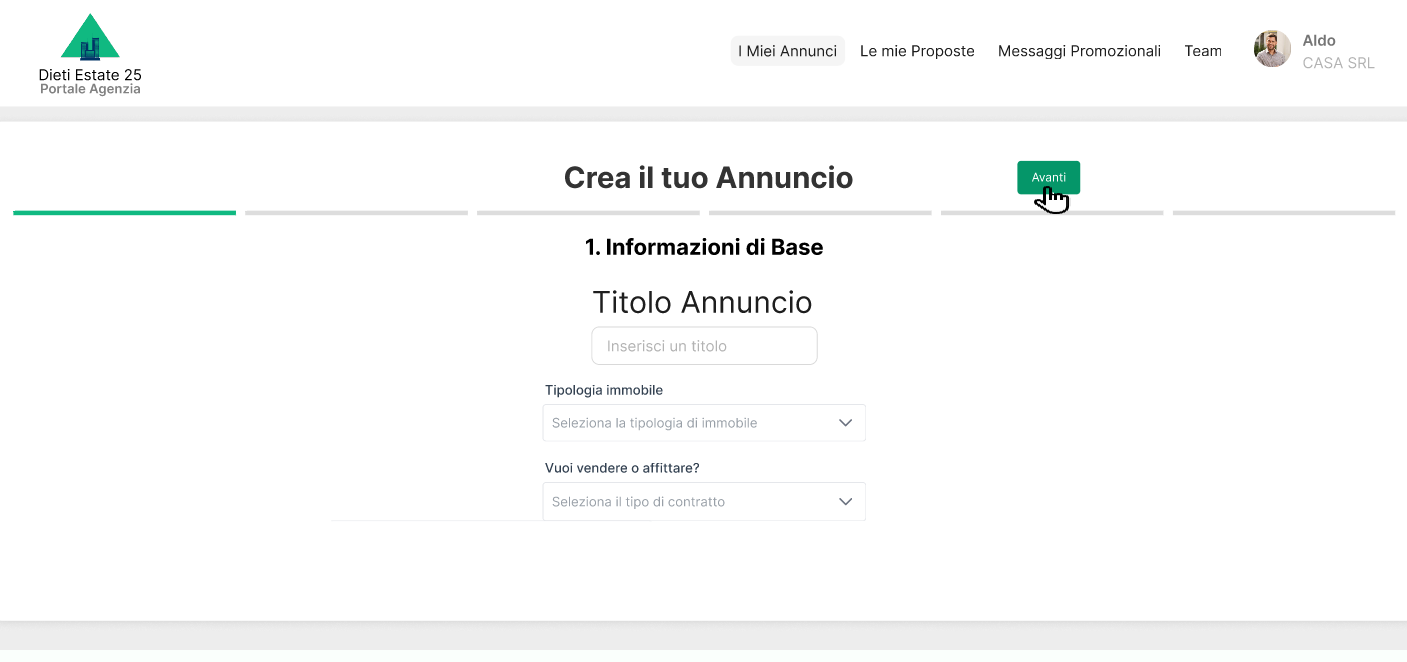
\includegraphics[width=0.7\textwidth]{Immagini/Mockup/aggiungi annuncio/scenario principale/step1.png} \\
                Cockburn: step 3
            \end{tabular}
        };
        
        % Nodo per immagine 2 con didascalia sotto, posizionato a destra di img1
        \node (img2) [below=of img1] {
            \begin{tabular}{c}
                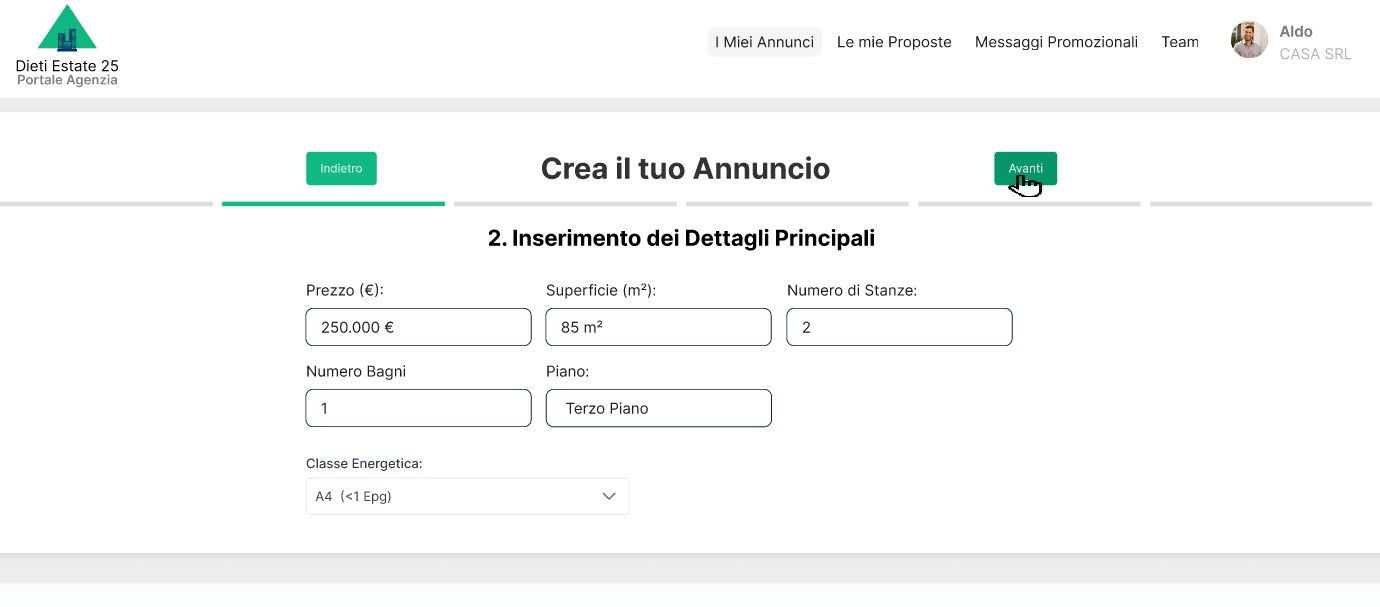
\includegraphics[width=0.7\textwidth]{Immagini/Mockup/aggiungi annuncio/scenario principale/step2.png} \\
                Cockburn: step4/5
            \end{tabular}
        };
        
        % Nodo per immagine 3 con didascalia sotto, posizionato sotto img2
        \node (img3) [below=of img2] {
            \begin{tabular}{c}
                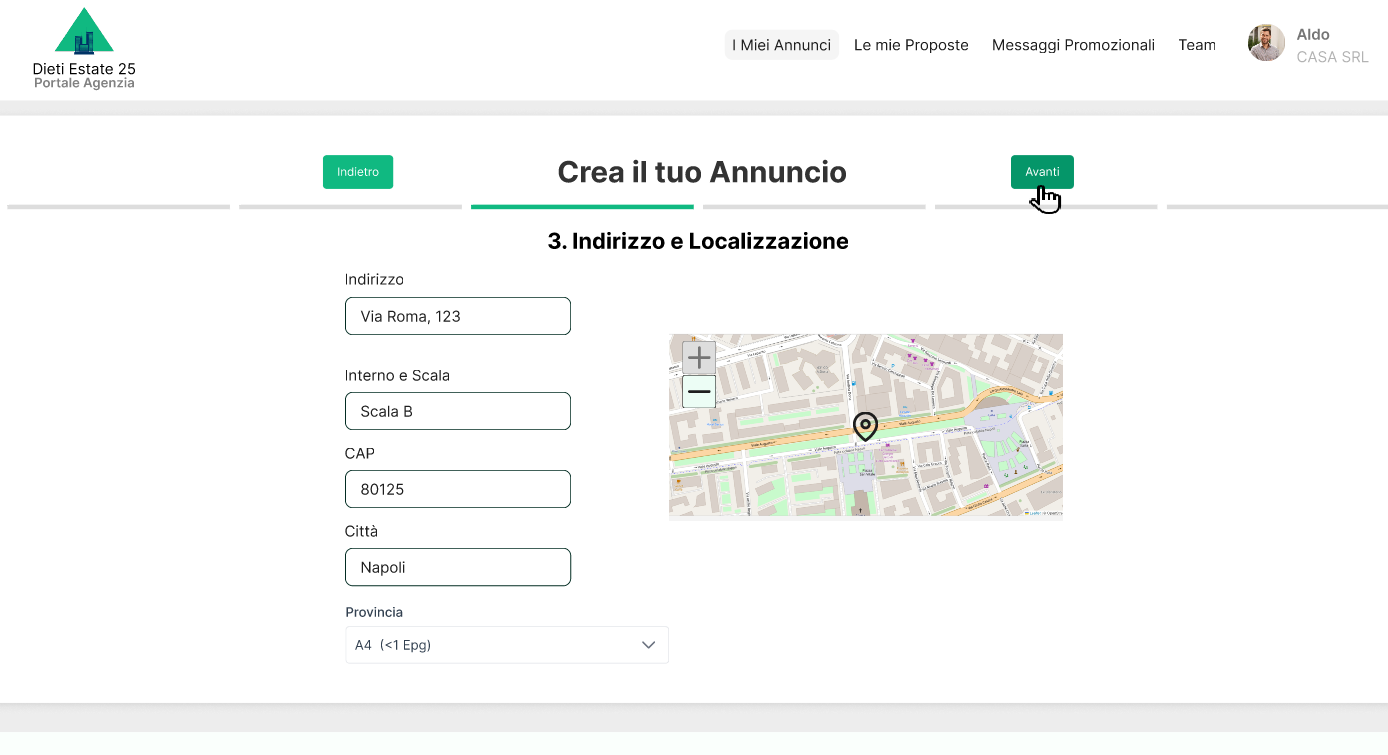
\includegraphics[width=0.7\textwidth]{Immagini/Mockup/aggiungi annuncio/scenario principale/step3.png} \\
                Cockburn: step 4/5
            \end{tabular}
        };
        
        % Disegna le frecce
        \draw[->, thick] (img1) -- (img2);
        \draw[->, thick] (img2) -- (img3);
      
    \end{tikzpicture}
    \caption{Mockup: scenario principale della tabella di Cockburn del caso d'uso nuovo annuncio.}
    \label{fig:mockup_scenario_principale_parte1_aggiungi_annuncio}
\end{figure}

\newpage



\begin{figure}[ht]
    \centering
    \begin{tikzpicture}[node distance=1.5cm and 1cm, auto]
        % Nodo per immagine 1 con didascalia sotto
        \node (img1) {
            \begin{tabular}{c}
                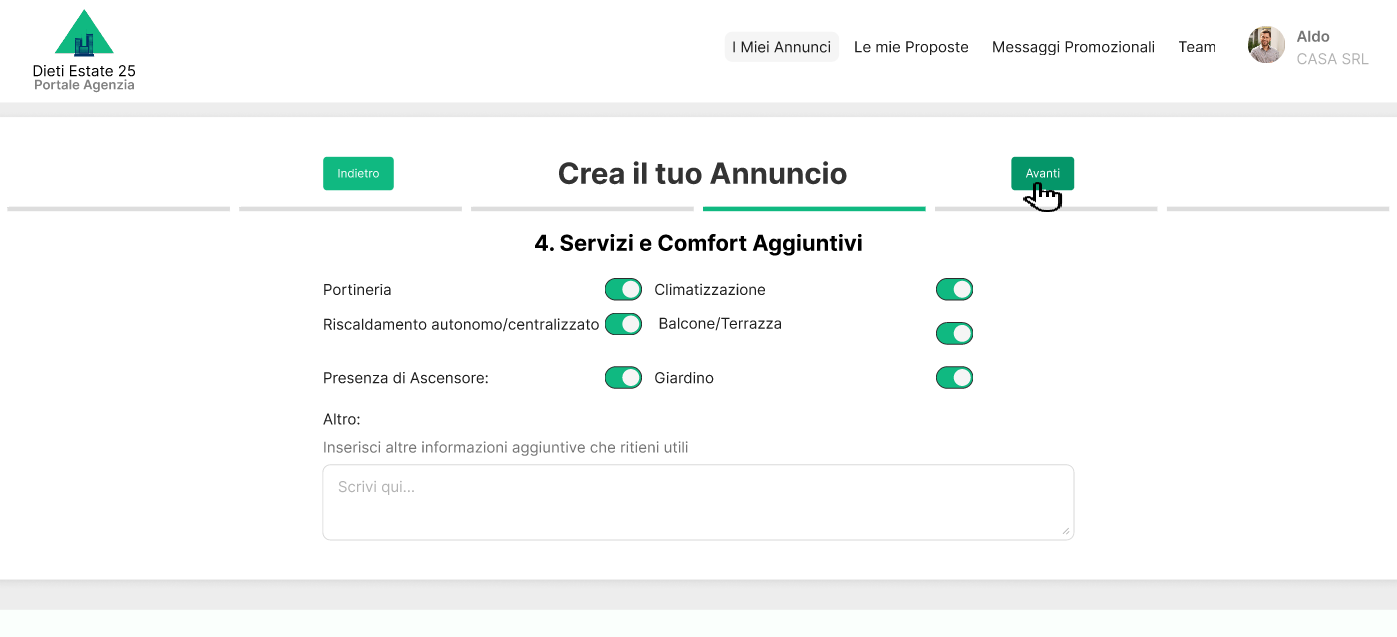
\includegraphics[width=\textwidth,keepaspectratio]{Immagini/Mockup/aggiungi annuncio/scenario principale/step4.png} \\
                Cockburn: step 4/5
            \end{tabular}
        };
        
        % Nodo per immagine 2 con didascalia sotto, posizionato a destra di img1
        \node (img2) [below=of img1] {
            \begin{tabular}{c}
                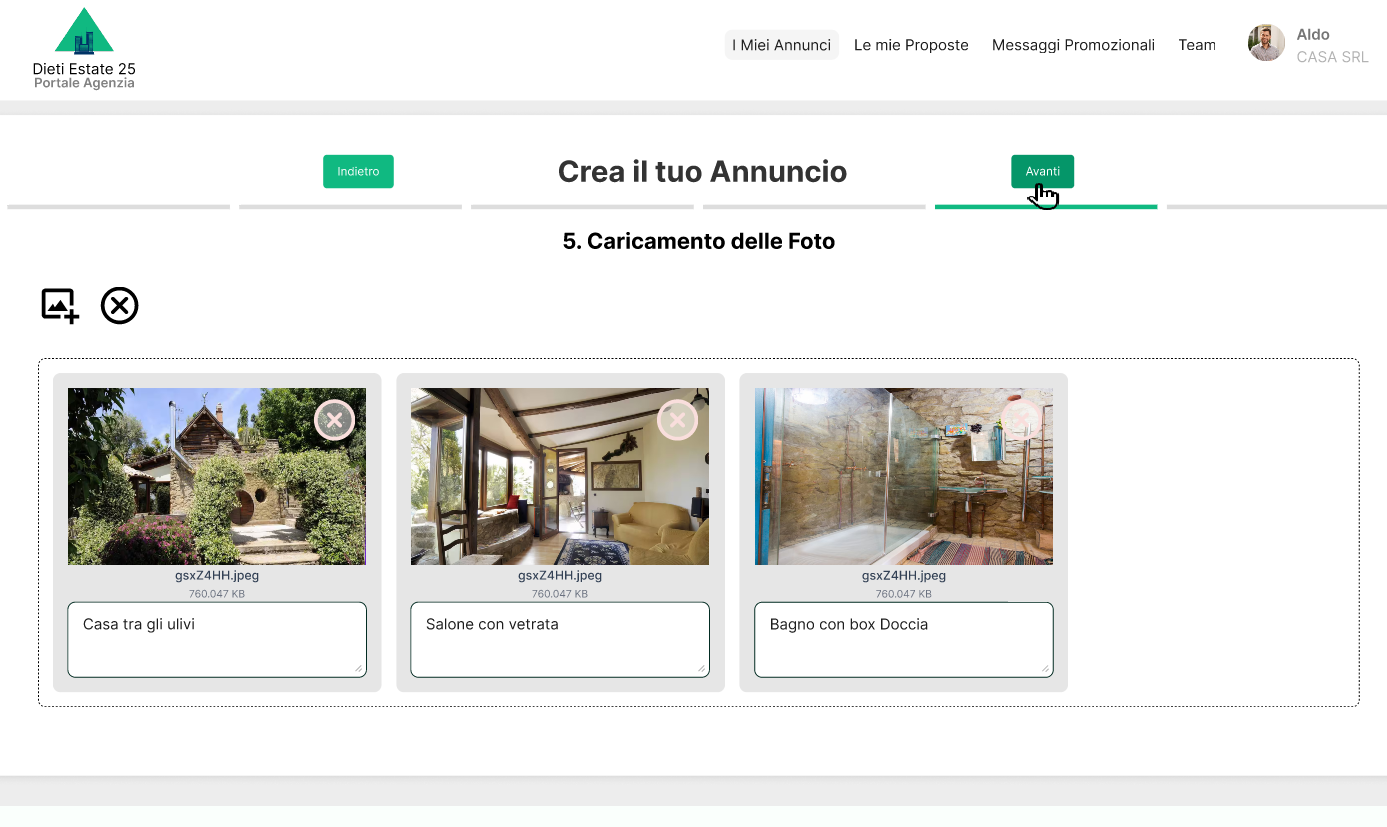
\includegraphics[width=\textwidth,keepaspectratio]{Immagini/Mockup/aggiungi annuncio/scenario principale/step5.png} \\
                Cockburn: step 6
            \end{tabular}
        };
        
        % Disegna le frecce
        \draw[->, thick] (img1) -- (img2);
      
    \end{tikzpicture}
    \caption{Mockup: scenario principale della tabella di Cockburn del caso d'uso nuovo annuncio.}
    \label{fig:tikz_flow}
\end{figure}

\newpage

\input{Requisiti Del Software/Analisi dei Requisiti/Mockup/aggiungi annuncio/scenario principale Parte III}



\clearpage
\newpage

\subsubsection{Estensione A: Disattivazione Notifiche dalla Visualizzazione di una Notifica}

Per offrire un maggiore controllo sulla gestione delle notifiche senza interrompere l’esperienza utente, il sistema permette di disattivare una categoria direttamente dalla visualizzazione di una notifica specifica. Questa variante è progettata per garantire una modifica consapevole delle preferenze, evitando azioni impulsive che potrebbero compromettere la ricezione di informazioni rilevanti.

\vspace{0.5cm}
\subsubsection{Interfaccia e Comportamento del Bottone}
Alla fine del testo di ogni notifica, se la relativa categoria è attiva, è presente un pulsante neutro con la dicitura “Disattiva notifiche”. Accanto al pulsante, un testo in grigio informa l’utente della funzione del pulsante, evitando ambiguità. L’utilizzo di colori non accesi e di un design discreto segue il principio della \textbf{gerarchia visiva} \cite{pieters2004}, scoraggiando azioni impulsive che potrebbero portare alla perdita involontaria di notifiche future.

\vspace{0.5cm}
\subsubsection{Modifica dello Stato e Feedback Visivo}
Quando l’utente clicca sul pulsante, il testo del pulsante cambia colore, diventando rosso, e il messaggio a fianco si aggiorna per sottolineare che la categoria di notifiche è stata disattivata. Questo utilizza il principio della \textbf{salienza visiva} \cite{nielsen1995}, enfatizzando il cambiamento e rendendo immediatamente chiara la conseguenza dell’azione.

\vspace{0.5cm}
\subsubsection{Incentivo alla Riattivazione}
Una volta disattivata una categoria tramite questa modalità, viene visualizzato un secondo pulsante con una call-to-action mirata per incentivare la riattivazione delle notifiche. Il design e il posizionamento del pulsante sfruttano il \textbf{principio dell’affordance} \cite{norman1988}, rendendo chiaro che l’utente ha la possibilità di tornare indietro sulla sua decisione in modo semplice e immediato.
\newline
Questa estensione si integra perfettamente con il modello generale di gestione delle notifiche, garantendo un’interazione fluida e coerente con le esigenze dell’utente. Nel caso in cui l’utente scelga di riattivare la categoria delle notifiche direttamente da una notifica, si passa all’\textbf{Estensione F}, che approfondisce questa modalità di gestione a partire dalle notifiche disattivate.
\begin{figure}[ht]
    \centering
    \begin{tikzpicture}[node distance=1.5cm and 1cm, auto]
        % Nodo per immagine 1 con didascalia sotto
        \node (img1) {
            \begin{tabular}{c}
                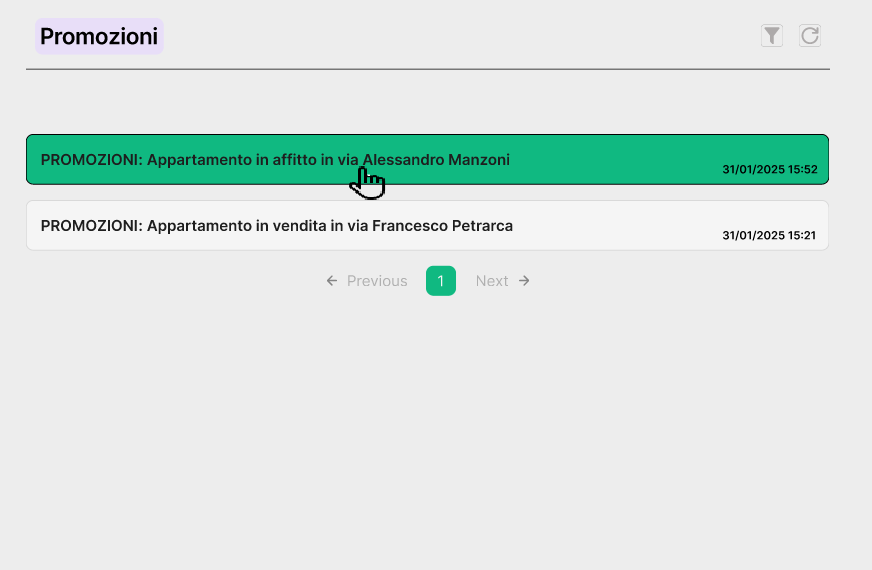
\includegraphics[width=0.4\textwidth]{Immagini/Mockup/notifiche/estensione A/clickNotifica.png} \\
                Cockburn: Extension A.2/A.3
            \end{tabular}
        };
        
        % Nodo per immagine 2 con didascalia sotto, posizionato a destra di img1
        \node (img2) [below=of img1] {
            \begin{tabular}{c}
                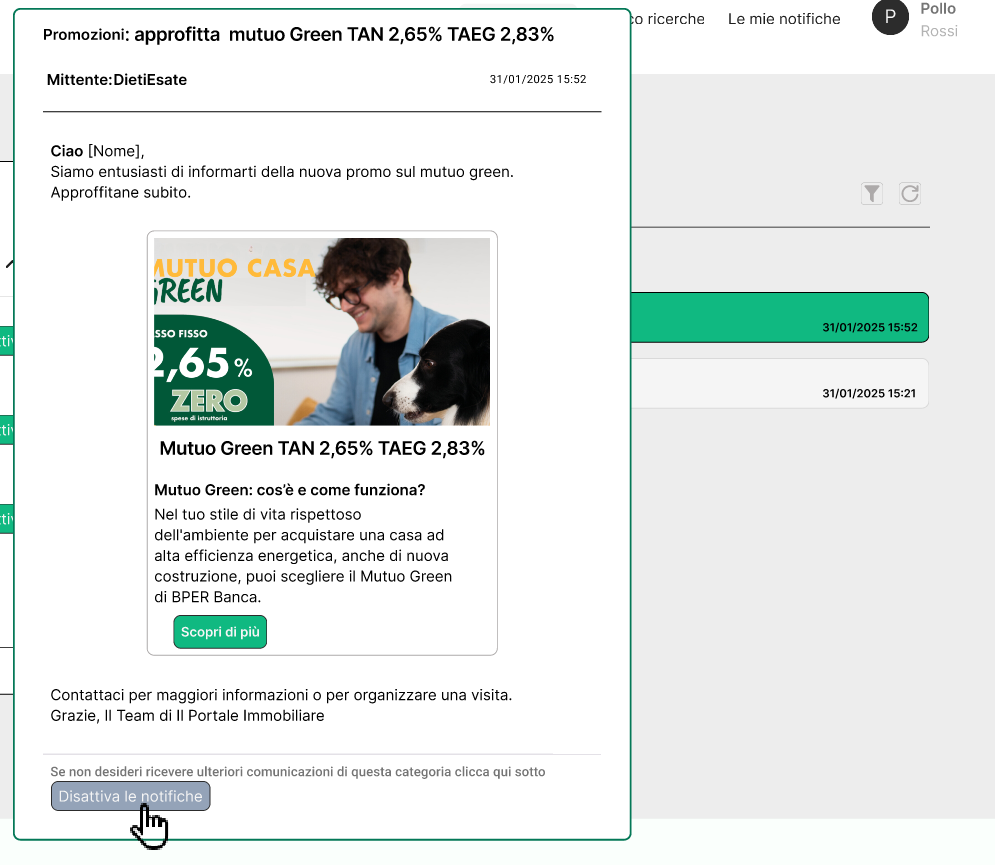
\includegraphics[width=0.4\textwidth]{Immagini/Mockup/notifiche/estensione A/clickDisattiva.png} \\
                Cockburn: Extension A.4
            \end{tabular}
        };
        
        % Nodo per immagine 3 con didascalia sotto, posizionato sotto img2
        \node (img3) [below=of img2] {
            \begin{tabular}{c}
                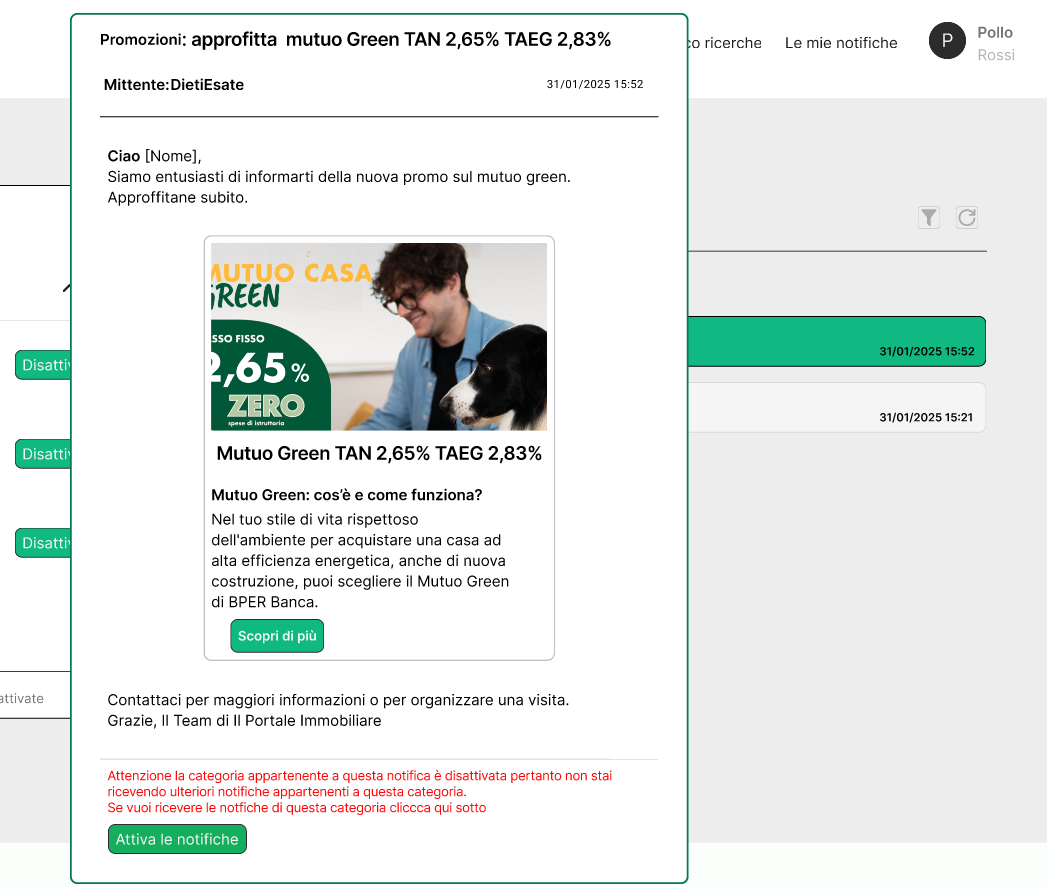
\includegraphics[width=0.4\textwidth]{Immagini/Mockup/notifiche/estensione A/disattivato.png} \\
                Cockburn: extension A.5
            \end{tabular}
        };
        
        % Disegna le frecce
        \draw[->, thick] (img1) -- (img2);
        \draw[->, thick] (img2) -- (img3);
      
    \end{tikzpicture}
    \caption{Mockup: estensione A della tabella di Cockburn del caso d'uso disattiva/attiva categoria notifica}
    \label{fig:mockup_estensione_A_disattiva_notifiche}
\end{figure}

\newpage



\clearpage
\newpage
\subsubsection{Estensione B: Ripristino di un Annuncio Precedente}
Se l’utente sceglie di \textbf{ripristinare l’annuncio precedente}, il sistema avvia un processo di caricamento per fornire un feedback visivo sulla ripresa dei dati. Sebbene i dati siano salvati localmente e il recupero sia immediato, un \textbf{indicatore di caricamento fittizio} viene mostrato per alcuni secondi prima di caricare la schermata.

Questa soluzione è basata sul principio della \textbf{coerenza con le aspettative dell’utente} \cite{shneiderman2004}. In un contesto digitale, un ripristino istantaneo potrebbe apparire innaturale e creare confusione. L’indicatore di caricamento:
\begin{itemize}
    \item Rafforza la percezione di un processo in corso, migliorando la trasparenza dell’operazione.
    \item Evita che l’utente si domandi se il recupero sia realmente avvenuto o se ci siano stati problemi tecnici.
    \item Contribuisce a una transizione più fluida tra stati dell’interfaccia.
\end{itemize}

Una volta completato il caricamento, il sistema presenta l’interfaccia con i dati precedentemente salvati, consentendo all’utente di riprendere il processo da dove era stato interrotto.


\begin{figure}[ht]
    \centering
    \begin{tikzpicture}[node distance=1.5cm and 1cm, auto]
        % Nodo per immagine 1 con didascalia sotto
        \node (img1) {
            \begin{tabular}{c}
                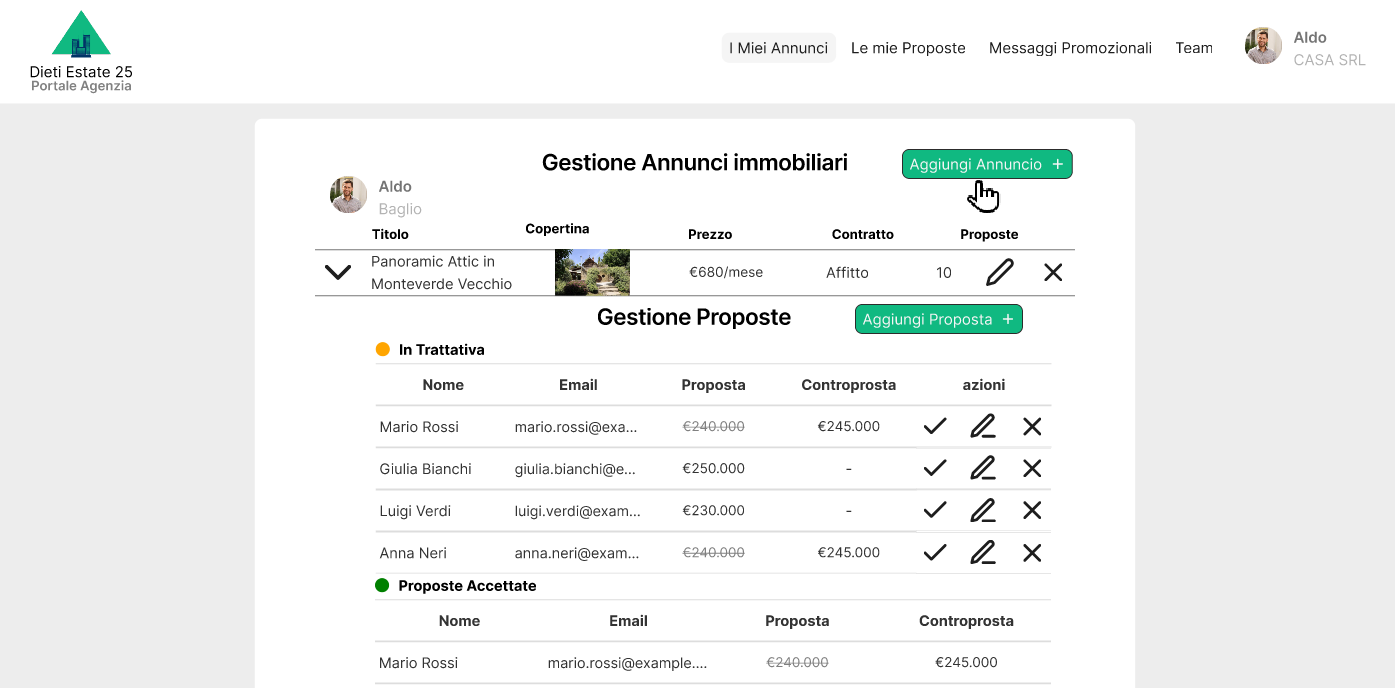
\includegraphics[width=0.7\textwidth]{Immagini/Mockup/aggiungi annuncio/estensione B/step1.png} \\
                click nuovo annuncio
            \end{tabular}
        };
        
        % Nodo per immagine 2 con didascalia sotto, posizionato a destra di img1
        \node (img2) [below=of img1] {
            \begin{tabular}{c}
                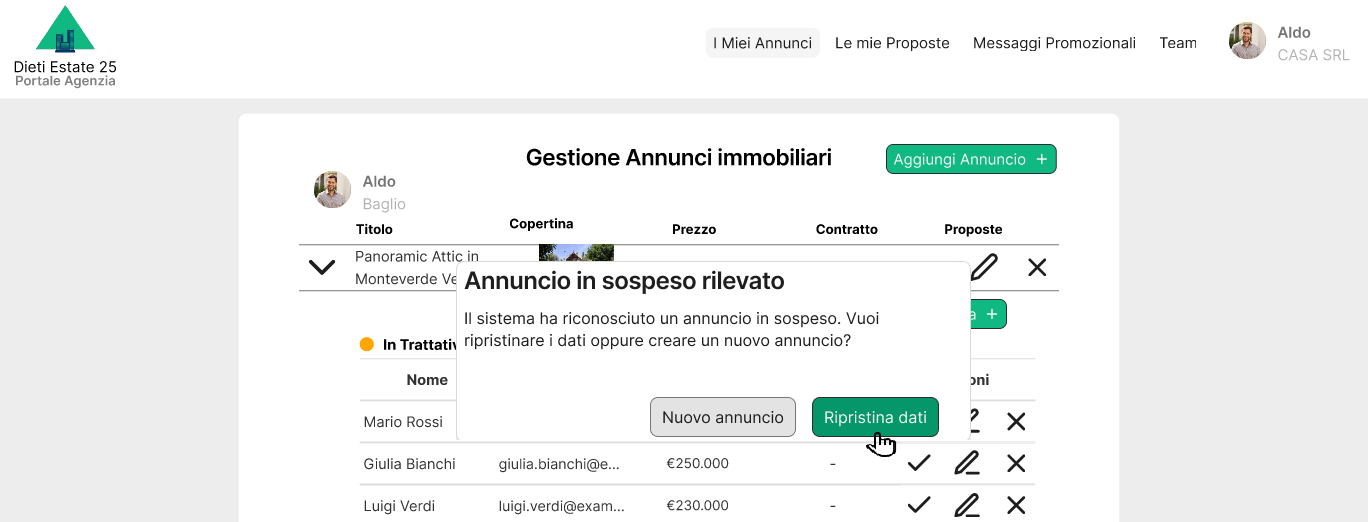
\includegraphics[width=0.7\textwidth]{Immagini/Mockup/aggiungi annuncio/estensione B/step2.png} \\
                Cockburn: extension B.2/B.3/B.4
            \end{tabular}
        };
        
        % Nodo per immagine 3 con didascalia sotto, posizionato sotto img2
        \node (img3) [below=of img2] {
            \begin{tabular}{c}
                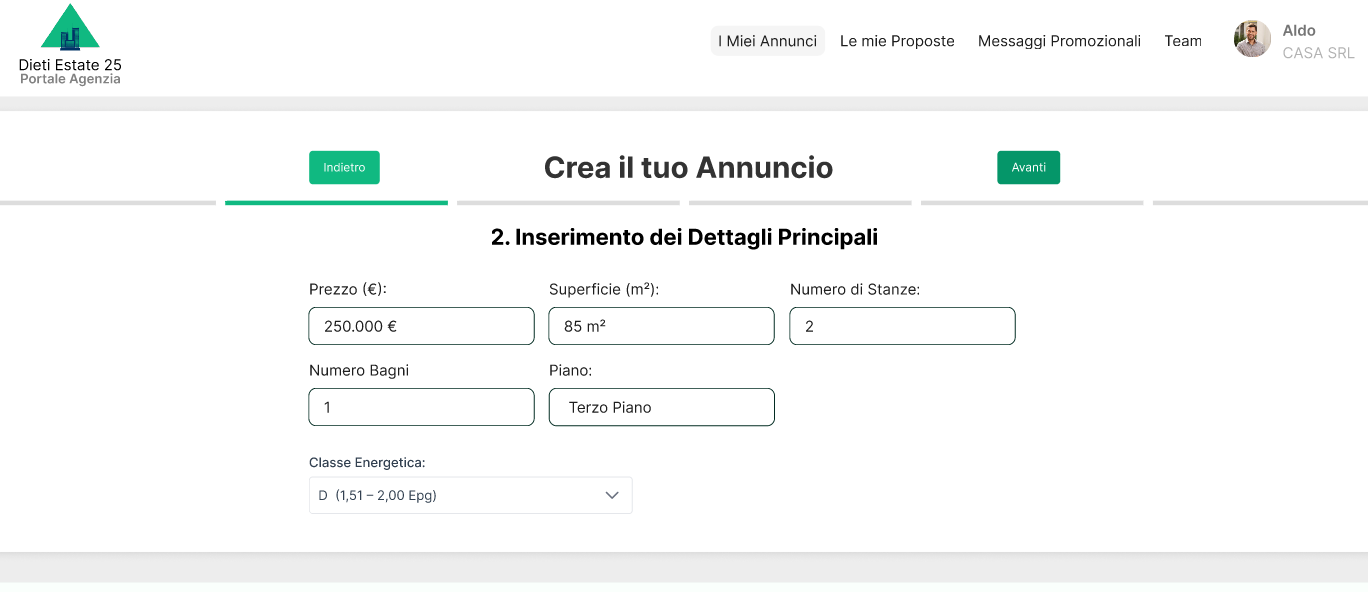
\includegraphics[width=0.7\textwidth]{Immagini/Mockup/aggiungi annuncio/estensione B/step3.png} \\
                Cockburn: extension B.5
            \end{tabular}
        };
        
        % Disegna le frecce
        \draw[->, thick] (img1) -- (img2);
        \draw[->, thick] (img2) -- (img3);
      
    \end{tikzpicture}
    \caption{Mockup: estensione B della tabella di Cockburn del caso d'uso nuovo annuncio}
    \label{fig:mockup_estensione_B_aggiungi_annuncio}
\end{figure}

\newpage




\clearpage
\newpage
\subsubsection{Estensione C: Errore Durante la Pubblicazione dell'Annuncio}

Nel caso in cui si verifichi un errore durante la pubblicazione dell'annuncio immobiliare, viene mostrato un popup informativo che comunica all'utente il problema riscontrato. Questo popup ha il compito di rassicurare l'utente che i dati inseriti non andranno persi, in quanto vengono salvati localmente, e invita a riprovare più tardi.

\subsubsection{Gestione dell'Errore e Feedback Utente}
Il popup presenta i seguenti elementi chiave:
\begin{itemize}
    \item \textbf{Messaggio chiaro e rassicurante}: informa l'utente dell'errore senza tecnicismi, riducendo il senso di frustrazione.
    \item \textbf{Pulsante “Riprova”}: consente di tentare nuovamente la pubblicazione con un'animazione di caricamento, per segnalare che l'azione è in corso e mantenere un senso di controllo e progressione.
    \item \textbf{Pulsante “Monstra i Dettagli”}: offre la possibilità di visualizzare l'errore tecnico riscontrato. Questa funzione segue i principi di trasparenza e controllo dell'utente, utili sia per utenti avanzati che per eventuali tecnici di supporto che potrebbero risolvere il problema più rapidamente.
\end{itemize}

\subsubsection{Principi di Design Applicati}
L'implementazione di questa gestione degli errori si basa su diversi principi della UX e dell'usabilità:
\begin{itemize}
    \item \textbf{Visibilità dello stato del sistema} \cite{nielsen1995}: l'animazione di caricamento fornisce un'indicazione chiara che il sistema sta lavorando sulla richiesta dell'utente.
    \item \textbf{Prevenzione degli errori} \cite{nielsen1995}: il salvataggio locale dei dati riduce la possibilità di perdere informazioni a causa di un problema temporaneo.
    \item \textbf{Fornire informazioni utili per il recupero dall'errore} \cite{nielsen1995}: il messaggio di errore è accompagnato da suggerimenti su come procedere e un'opzione per visualizzare i dettagli tecnici, utile per il supporto tecnico.
\end{itemize}

Queste soluzioni mirano a mantenere un'esperienza utente fluida e priva di frustrazione, minimizzando il disagio derivante da problemi tecnici imprevisti.


\begin{figure}[ht]
    \centering
    \begin{tikzpicture}[node distance=1.5cm and 1cm, auto]
        % Nodo per immagine 1 con didascalia sotto
        \node (img1) {
            \begin{tabular}{c}
                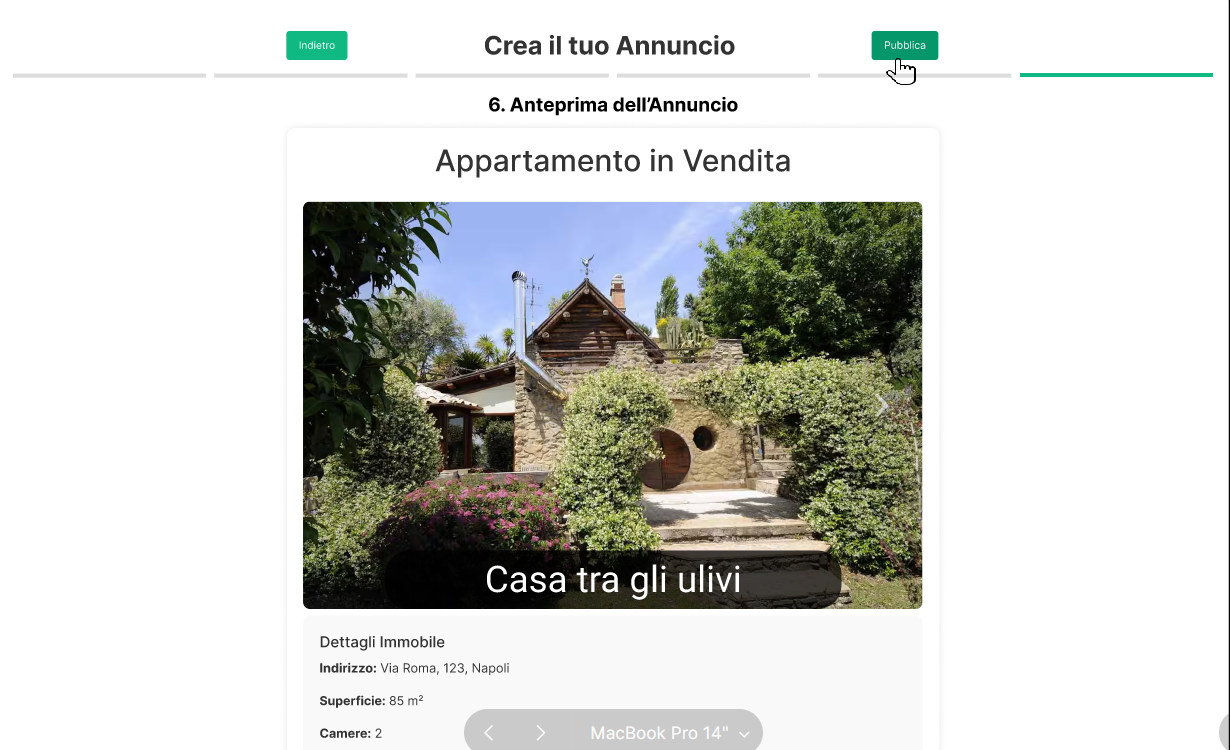
\includegraphics[width=0.7\textwidth]{Immagini/Mockup/aggiungi annuncio/estensione C/step1.png} \\
                click pubblica nuovo annuncio
            \end{tabular}
        };
        
        % Nodo per immagine 2 con didascalia sotto, posizionato a destra di img1
        \node (img2) [below=of img1] {
            \begin{tabular}{c}
                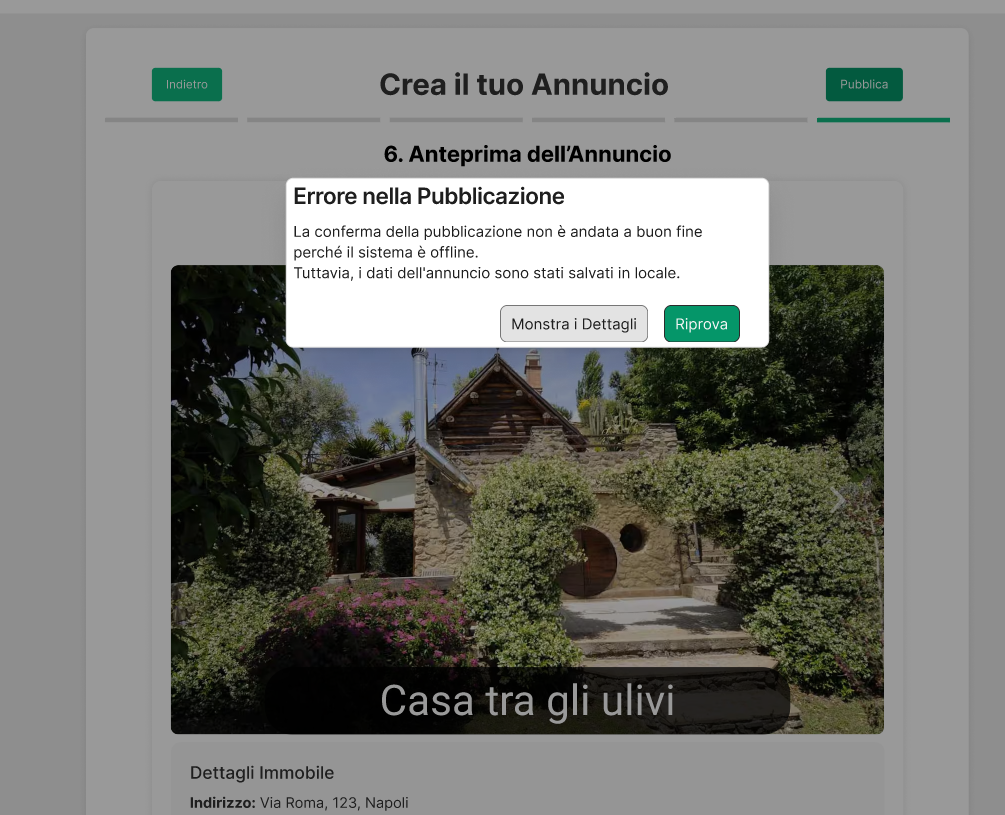
\includegraphics[width=\textwidth]{Immagini/Mockup/aggiungi annuncio/estensione C/step2.png} \\
                Cockburn: extension C.9/C.10
            \end{tabular}
        };
        
        
        % Disegna le frecce
        \draw[->, thick] (img1) -- (img2);
      
    \end{tikzpicture}
    \caption{Mockup: estensione C della tabella di Cockburn del caso d'uso nuovo annuncio}
    \label{fig:tikz_flow}
\end{figure}

\newpage



\clearpage
\newpage

\subsubsection{Estensione D: Modifica Rapida dello Stato delle Notifiche con Attivazione Immediata}

Questa variante rappresenta l’approccio duale dell’\textbf{Estensione C}, semplificando ulteriormente l’attivazione delle notifiche. L’obiettivo è ridurre i passaggi necessari per riattivare una categoria disattivata, mantenendo comunque un controllo chiaro sulla disattivazione.

\vspace{0.5cm}
\subsubsection{Interfaccia e Interazione}
Analogamente all’\textbf{Estensione C}, ogni categoria nella barra laterale dispone di un pulsante contestuale per modificarne lo stato. Il pulsante può assumere due stati:

\begin{itemize}
    \item \textbf{Attiva}, se la categoria è attualmente disabilitata.
    \item \textbf{Disattiva}, se la categoria è attualmente abilitata.
\end{itemize}

Le interazioni dell’utente variano a seconda dell’azione eseguita:

\begin{itemize}
    \item \textbf{Disattivazione di una categoria}:
    \begin{itemize}
        \item Al clic su \textbf{Disattiva}, appare un popup di conferma che informa l’utente sulle conseguenze della scelta, prevenendo azioni accidentali in linea con i principi di Nielsen \cite{nielsen1995}.
        \item Se confermata, la categoria viene spostata nella sezione delle notifiche disattivate tramite un’animazione di transizione.
        \item Il pulsante cambia stato, diventando \textbf{Attiva}, fornendo un feedback visivo chiaro sulla modifica.
    \end{itemize}
    
    \item \textbf{Attivazione di una categoria}:
    \begin{itemize}
        \item Al clic su \textbf{Attiva}, il sistema aggiorna immediatamente lo stato della notifica senza richiedere una conferma esplicita.
        \item La categoria viene spostata nella sezione delle notifiche attive con un’animazione fluida, applicando il principio della \textbf{gestalt della continuità} \cite{miller1956}.
        \item Il pulsante cambia stato in \textbf{Disattiva}, rendendo la modifica evidente e intuitiva.
    \end{itemize}
\end{itemize}

\subsubsection{Feedback Visivo e UX Design}
L’esperienza utente è ottimizzata tramite tecniche di design che garantiscono chiarezza e immediatezza:

\begin{itemize}
    \item \textbf{Popup di conferma per la disattivazione}: aiuta a prevenire errori e rende consapevole l’utente delle conseguenze della scelta \cite{nielsen1995}.
    \item \textbf{Animazione di transizione}: assicura una continuità visiva fluida nello spostamento delle categorie, migliorando la percezione del cambiamento \cite{miller1956}.
    \item \textbf{Aggiornamento immediato dello stato del pulsante}: il cambio di testo e colore riflette lo stato corrente della categoria, riducendo l’ambiguità e migliorando la prevedibilità dell’interazione.
\end{itemize}

Questa estensione semplifica l’attivazione delle notifiche, eliminando il passaggio della conferma e migliorando la fluidità dell’interazione, senza compromettere il controllo dell’utente sulla gestione delle proprie preferenze.

\begin{figure}[ht]
    \centering
    \begin{tikzpicture}[node distance=1.5cm and 1cm, auto]
        % Nodo per immagine 1 con didascalia sotto
        \node (img1) {
            \begin{tabular}{c}
                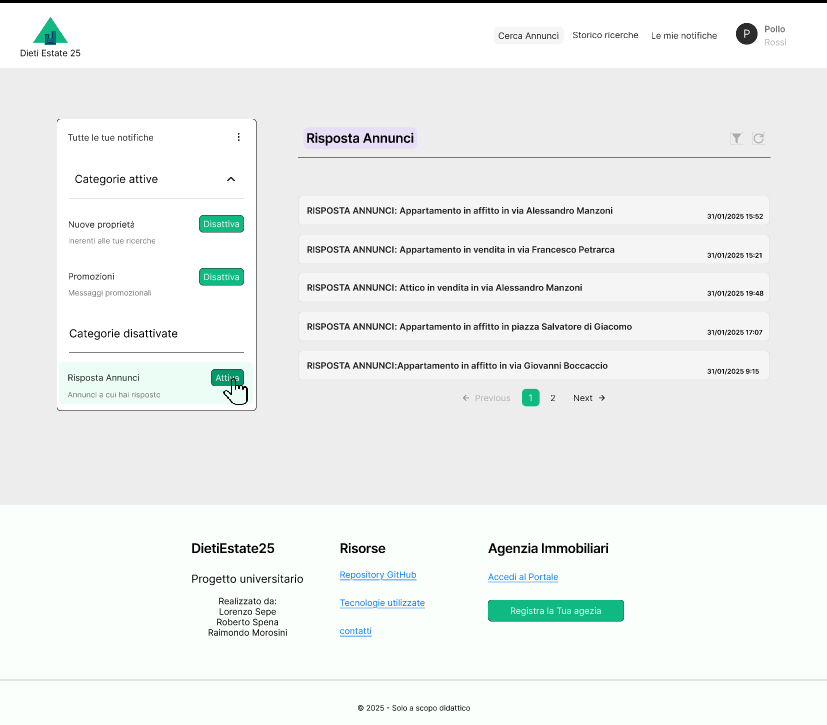
\includegraphics[width=0.6\textwidth]{Immagini/Mockup/notifiche/estensione D/clickAttiva.png} \\
                Cockburn: Extension D.2
            \end{tabular}
        };
        
        % Nodo per immagine 2 con didascalia sotto, posizionato a destra di img1
        \node (img2) [below=of img1] {
            \begin{tabular}{c}
                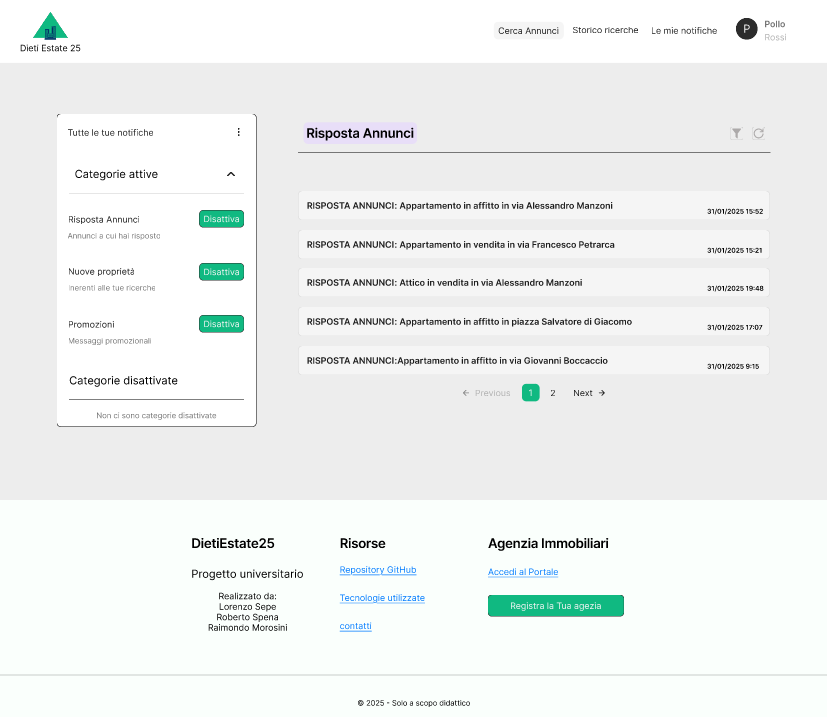
\includegraphics[width=0.6\textwidth]{Immagini/Mockup/notifiche/estensione D/attivato.png} \\
                Cockburn: step 8/9/10
            \end{tabular}
        };
        
        % Disegna le frecce
        \draw[->, thick] (img1) -- (img2);
      
    \end{tikzpicture}
    \caption{Mockup: estensione D della tabella di Cockburn del caso d'uso disattiva/attiva categoria notifica}
    \label{fig:mockup_estensione_D_disattiva_notifiche}
\end{figure}

\newpage



\clearpage
\newpage

\subsection{Caso d'Uso: Attivazione e Disattivazione Notifiche}

Il sistema prevede un'interfaccia dedicata alla gestione delle preferenze di notifica, pensata per permettere all'utente di curare la propria esperienza d'uso dell'applicazione, ricevendo news solo sugli argomenti di interesse.\\
In questa sezione andremo a esaminare le scelte effettuate durante la progettazione, l'impatto sull'esperienza utente e i prototipi generati alla fine dell'analisi. 

\vspace{0.5cm}
\subsubsection{Tipologie di Notifiche e Controllo Utente}
Le notifiche sono suddivise in diverse categorie per permettere una personalizzazione granulare:
\begin{itemize}
    \item \textbf{Annunci di nuovi immobili}: notifiche basate sulle ricerche dell’utente.
    \item \textbf{Risposte alle offerte}: aggiornamenti sulle interazioni con gli annunci pubblicati.
    \item \textbf{Messaggi promozionali}: comunicazioni di marketing e offerte esclusive.
\end{itemize}
L’utente può, in qualsiasi momento, disattivare le notifiche per una o più categorie, mantenendo un controllo totale sulla propria esperienza \cite{shneiderman2004}.

\vspace{0.5cm}
\subsubsection{Gestione delle Notifiche e Conferma delle Modifiche}
La gestione delle notifiche avviene principalmente attraverso la schermata delle notifiche, composta da:
\begin{itemize}
    \item \textbf{Lista delle notifiche ricevute}, ognuna cliccabile per visualizzare i dettagli.
    \item \textbf{Barra laterale con le categorie di notifiche}, suddivise in:
    \begin{itemize}
        \item \textbf{Categorie attive}, con notifiche attualmente abilitate.
        \item \textbf{Categorie disattivate}, che non inviano più notifiche.
    \end{itemize}
\end{itemize}

In cima alla barra laterale è presente un’icona che, se cliccata, apre una schermata popup intitolata “Attiva e Disattiva Notifiche”. All’interno, ogni categoria è rappresentata da un toggle switch che indica lo stato attuale delle notifiche.

\vspace{0.5cm}
\subsubsection{Feedback Visivo e Animazioni Intuitive}
Per garantire un’interazione chiara e immediata, il sistema utilizza diverse tecniche di UX design:
\begin{itemize}
    \item \textbf{Animazione di transizione}: quando un toggle viene modificato, la categoria si sposta visivamente tra la sezione attiva e quella disattiva, sfruttando il principio di \textbf{gestalt della continuità} \cite{miller1956} per rendere il cambiamento intuitivo.
    \item \textbf{Feedback visivo immediato}: l’utente percepisce immediatamente l’effetto dell’azione senza necessità di un testo esplicativo eccessivo.
\end{itemize}

\newpage
\subsubsection{Conferma e Implicazioni della Disattivazione}
Per evitare errori accidentali e garantire consapevolezza delle conseguenze, la disattivazione di una categoria di notifiche è accompagnata da:
\begin{itemize}
    \item Un popup di conferma che informa l’utente che, durante il periodo in cui le notifiche sono disattivate, le notifiche non potranno essere recuperate \cite{wickens2008}.
    \item Un ulteriore messaggio di avviso prima della conferma definitiva, in linea con le \textbf{heuristiche di usabilità di Nielsen} \cite{nielsen1995} per la prevenzione degli errori.
\end{itemize}

Solo dopo la conferma finale, il sistema applica le modifiche alle preferenze dell'utente, garantendo un'interazione consapevole e trasparente.\\
Nel prototipo questi comportamenti sono stati modellati con un pulsante, tuttavia nell'applicazione finale è stato deciso di sostituirlo con un menù contestuale.



\begin{figure}[ht]
    \centering
    \begin{tikzpicture}[node distance=1.5cm and 1cm, auto]
        % Nodo per immagine 1 con didascalia sotto
        \node (img1) {
            \begin{tabular}{c}
                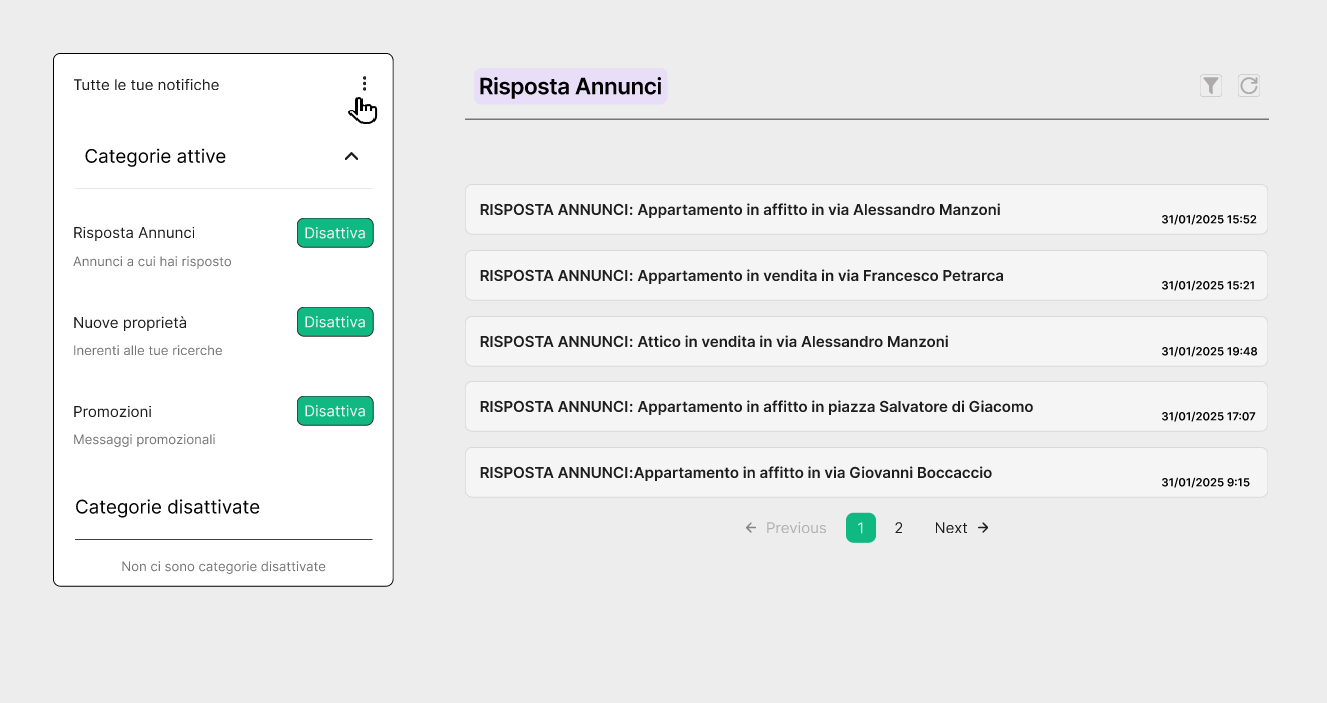
\includegraphics[width=0.7\textwidth]{Immagini/Mockup/notifiche/scenario principale/Pagina Lista Notifiche.png}\\
                Cockburn: step 1/2/3
            \end{tabular}
        };
        
        % Nodo per immagine 2 con didascalia sotto, posizionato a destra di img1
        \node (img2) [below=of img1] {
            \begin{tabular}{c}
                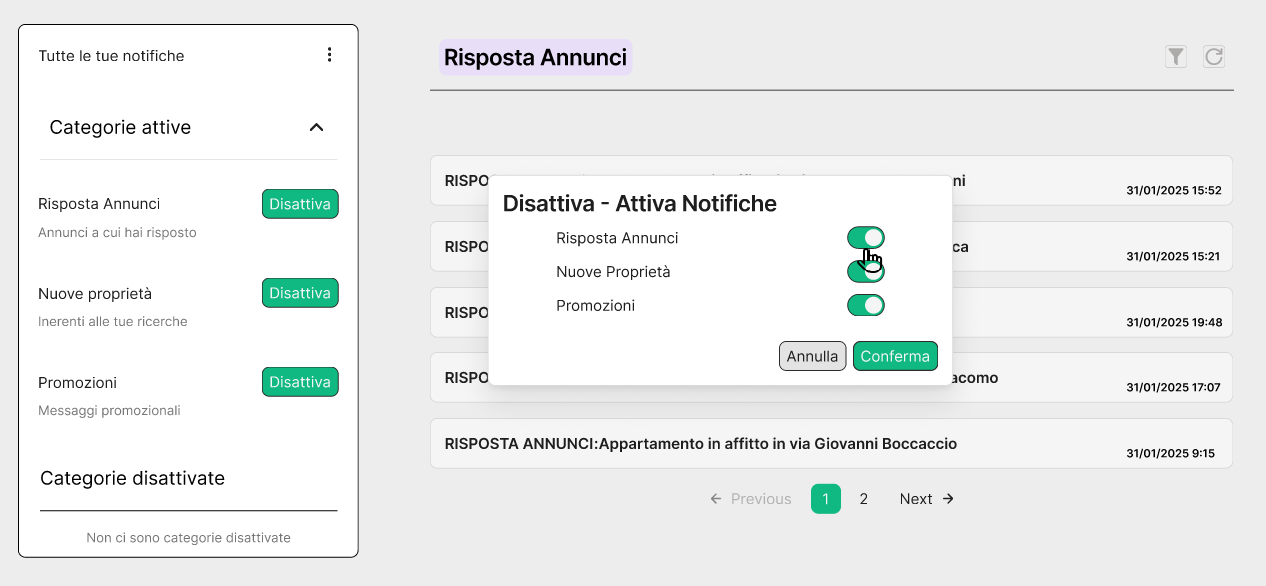
\includegraphics[width=0.7\textwidth]{Immagini/Mockup/notifiche/scenario principale/perDisattivareRisposte.png} \\
                Cockburn: step 4
            \end{tabular}
        };
        
        % Nodo per immagine 3 con didascalia sotto, posizionato sotto img2
        \node (img3) [below=of img2] {
            \begin{tabular}{c}
                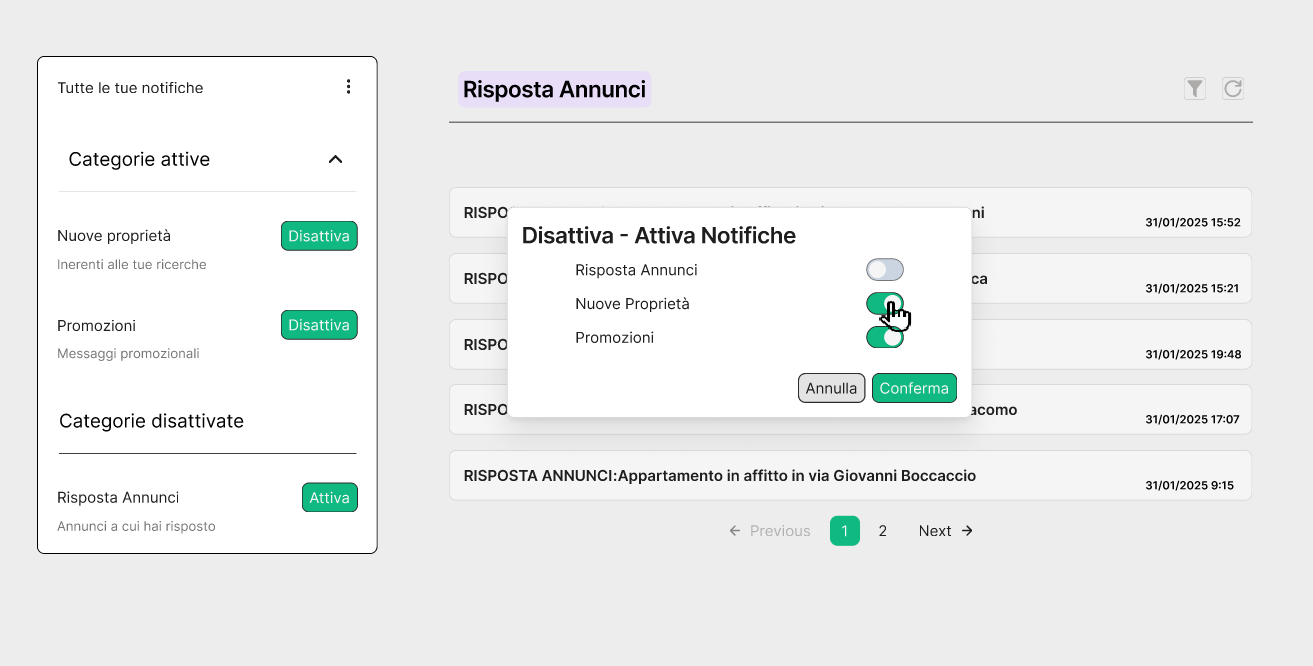
\includegraphics[width=0.7\textwidth]{Immagini/Mockup/notifiche/scenario principale/perDisattivareNueve.png} \\
                Cockburn: step 4
            \end{tabular}
        };

        
        % Disegna le frecce
        \draw[->, thick] (img1) -- (img2);
        \draw[->, thick] (img2) -- (img3);
        
    \end{tikzpicture}
    \caption{Mockup: scenario principale della tabella di Cockburn del caso d'uso disattiva/attiva categoria notifica}
    \label{fig:mockup_scenario_principale_parte1_disattiva_notifiche}
\end{figure}

\clearpage
\newpage

\begin{figure}[ht]
    \centering
    \begin{tikzpicture}[node distance=1.5cm and 1cm, auto]
      

         \node (img4){
            \begin{tabular}{c}
                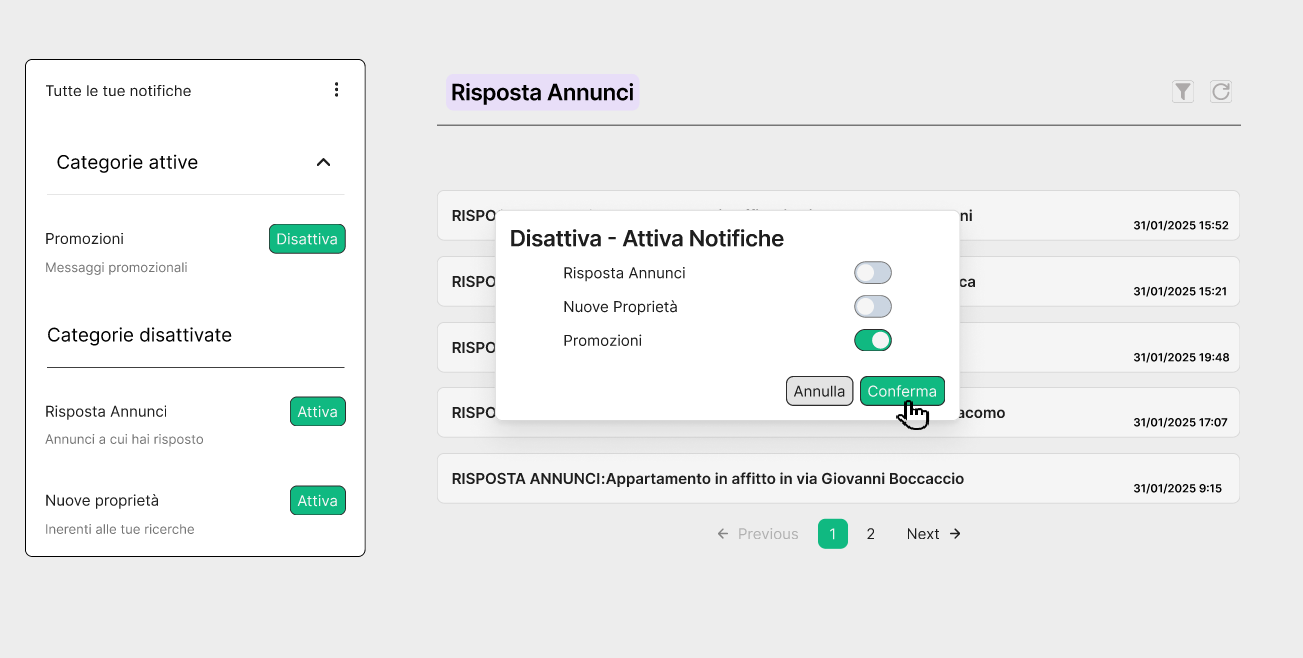
\includegraphics[width=0.7\textwidth]{Immagini/Mockup/notifiche/scenario principale/clickConferma.png} \\
                Cockburn: step 5
            \end{tabular}
        };

        \node (img5) [below=of img4] {
            \begin{tabular}{c}
                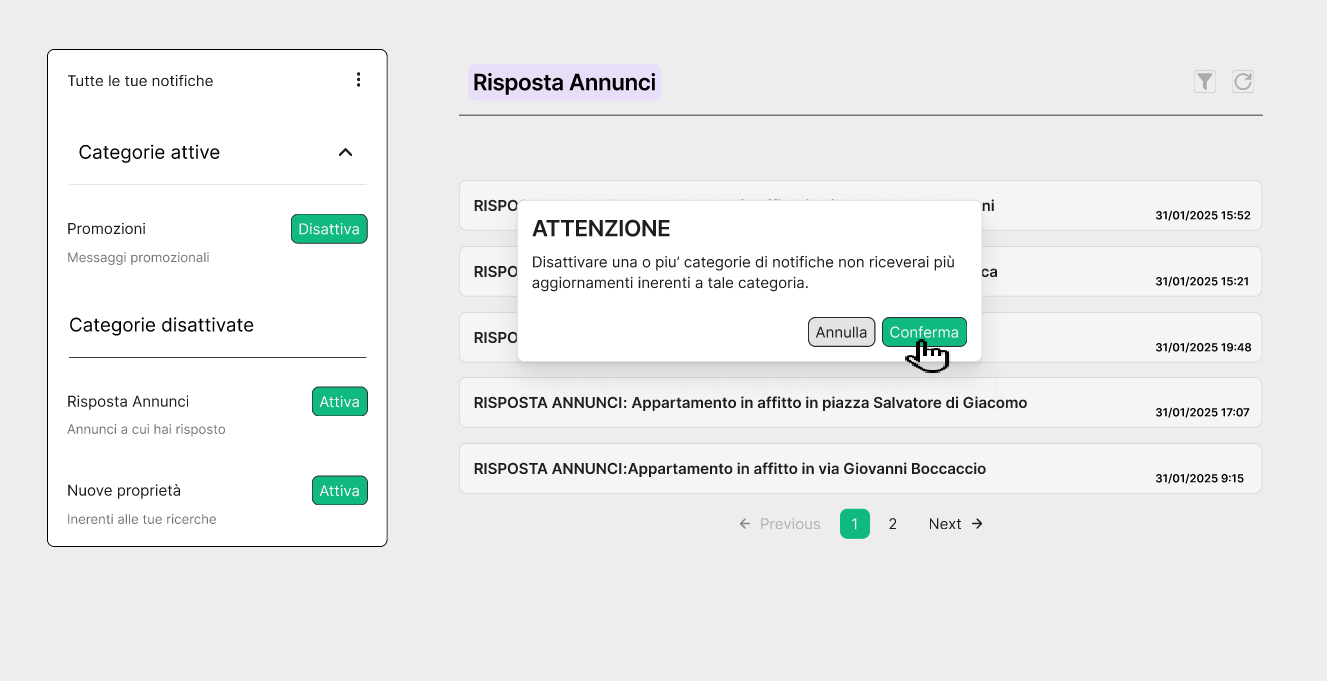
\includegraphics[width=0.7\textwidth]{Immagini/Mockup/notifiche/scenario principale/allerAvvisoDisattivazione.png} \\
                Cockburn: step 6/7
            \end{tabular}
        };

        \node (img6) [below=of img5] {
            \begin{tabular}{c}
                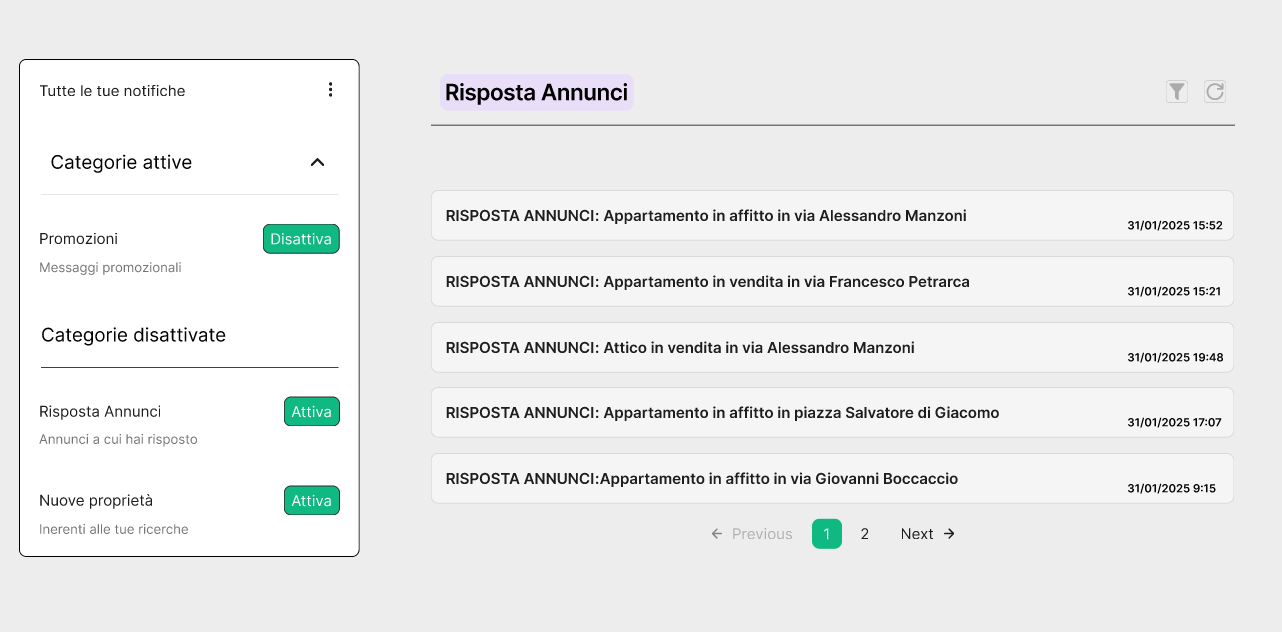
\includegraphics[width=0.7\textwidth]{Immagini/Mockup/notifiche/scenario principale/ScenarioPrincipaleCompletato.png} \\
                Conckburn: step 8/9/10
            \end{tabular}
        };
        
        % Disegna le frecce
        \draw[->, thick] (img4) -- (img5);
        \draw[->, thick] (img5) -- (img6);
        
    \end{tikzpicture}
    \caption{Parte 2 mockup: scenario principale della tabella di Cockburn del caso d'uso disattiva/attiva categoria notifica}
    \label{fig:mockup_scenario_principale_parte2_disattiva_notifiche}
\end{figure}

\clearpage
\newpage

\subsubsection{Estensione A: Disattivazione Notifiche dalla Visualizzazione di una Notifica}

Per offrire un maggiore controllo sulla gestione delle notifiche senza interrompere l’esperienza utente, il sistema permette di disattivare una categoria direttamente dalla visualizzazione di una notifica specifica. Questa variante è progettata per garantire una modifica consapevole delle preferenze, evitando azioni impulsive che potrebbero compromettere la ricezione di informazioni rilevanti.

\vspace{0.5cm}
\subsubsection{Interfaccia e Comportamento del Bottone}
Alla fine del testo di ogni notifica, se la relativa categoria è attiva, è presente un pulsante neutro con la dicitura “Disattiva notifiche”. Accanto al pulsante, un testo in grigio informa l’utente della funzione del pulsante, evitando ambiguità. L’utilizzo di colori non accesi e di un design discreto segue il principio della \textbf{gerarchia visiva} \cite{pieters2004}, scoraggiando azioni impulsive che potrebbero portare alla perdita involontaria di notifiche future.

\vspace{0.5cm}
\subsubsection{Modifica dello Stato e Feedback Visivo}
Quando l’utente clicca sul pulsante, il testo del pulsante cambia colore, diventando rosso, e il messaggio a fianco si aggiorna per sottolineare che la categoria di notifiche è stata disattivata. Questo utilizza il principio della \textbf{salienza visiva} \cite{nielsen1995}, enfatizzando il cambiamento e rendendo immediatamente chiara la conseguenza dell’azione.

\vspace{0.5cm}
\subsubsection{Incentivo alla Riattivazione}
Una volta disattivata una categoria tramite questa modalità, viene visualizzato un secondo pulsante con una call-to-action mirata per incentivare la riattivazione delle notifiche. Il design e il posizionamento del pulsante sfruttano il \textbf{principio dell’affordance} \cite{norman1988}, rendendo chiaro che l’utente ha la possibilità di tornare indietro sulla sua decisione in modo semplice e immediato.
\newline
Questa estensione si integra perfettamente con il modello generale di gestione delle notifiche, garantendo un’interazione fluida e coerente con le esigenze dell’utente. Nel caso in cui l’utente scelga di riattivare la categoria delle notifiche direttamente da una notifica, si passa all’\textbf{Estensione F}, che approfondisce questa modalità di gestione a partire dalle notifiche disattivate.
\begin{figure}[ht]
    \centering
    \begin{tikzpicture}[node distance=1.5cm and 1cm, auto]
        % Nodo per immagine 1 con didascalia sotto
        \node (img1) {
            \begin{tabular}{c}
                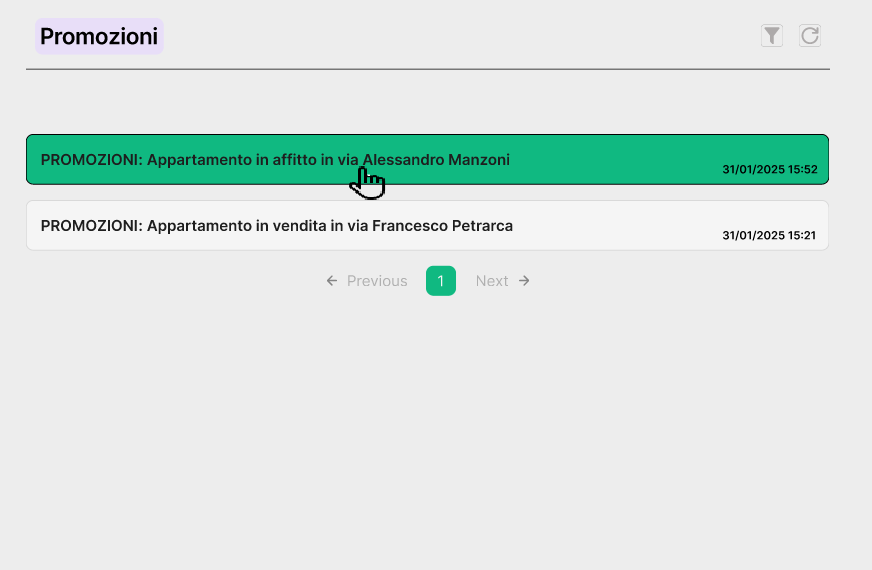
\includegraphics[width=0.4\textwidth]{Immagini/Mockup/notifiche/estensione A/clickNotifica.png} \\
                Cockburn: Extension A.2/A.3
            \end{tabular}
        };
        
        % Nodo per immagine 2 con didascalia sotto, posizionato a destra di img1
        \node (img2) [below=of img1] {
            \begin{tabular}{c}
                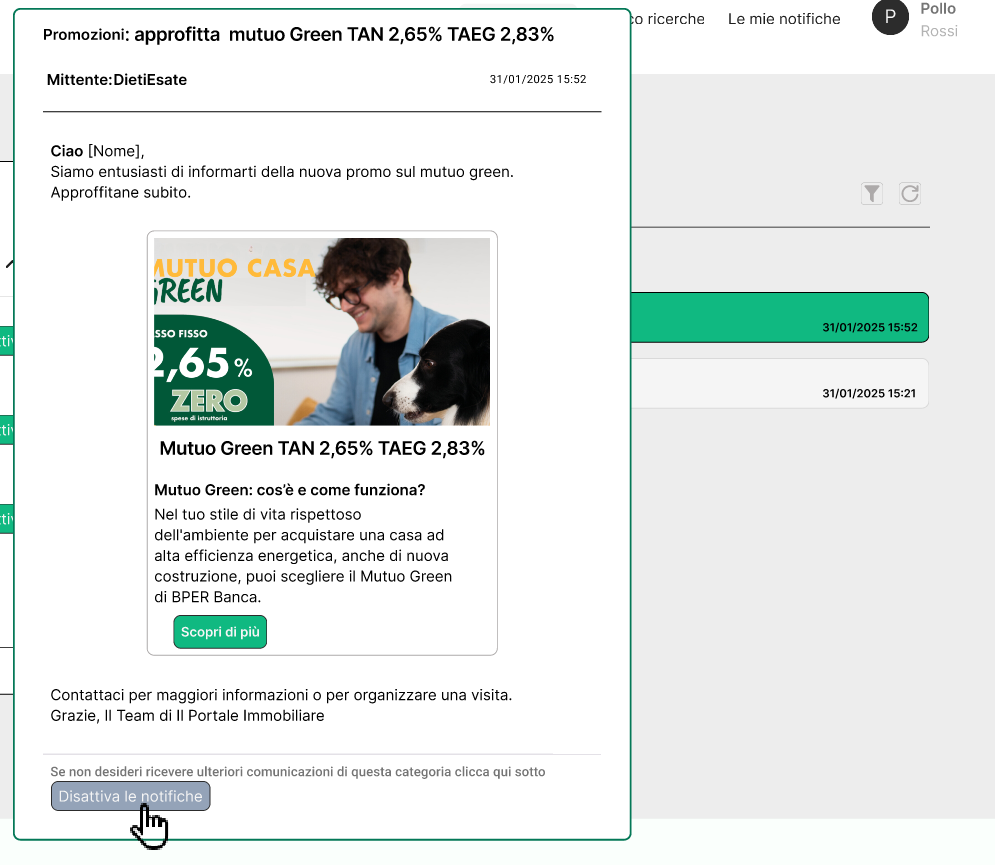
\includegraphics[width=0.4\textwidth]{Immagini/Mockup/notifiche/estensione A/clickDisattiva.png} \\
                Cockburn: Extension A.4
            \end{tabular}
        };
        
        % Nodo per immagine 3 con didascalia sotto, posizionato sotto img2
        \node (img3) [below=of img2] {
            \begin{tabular}{c}
                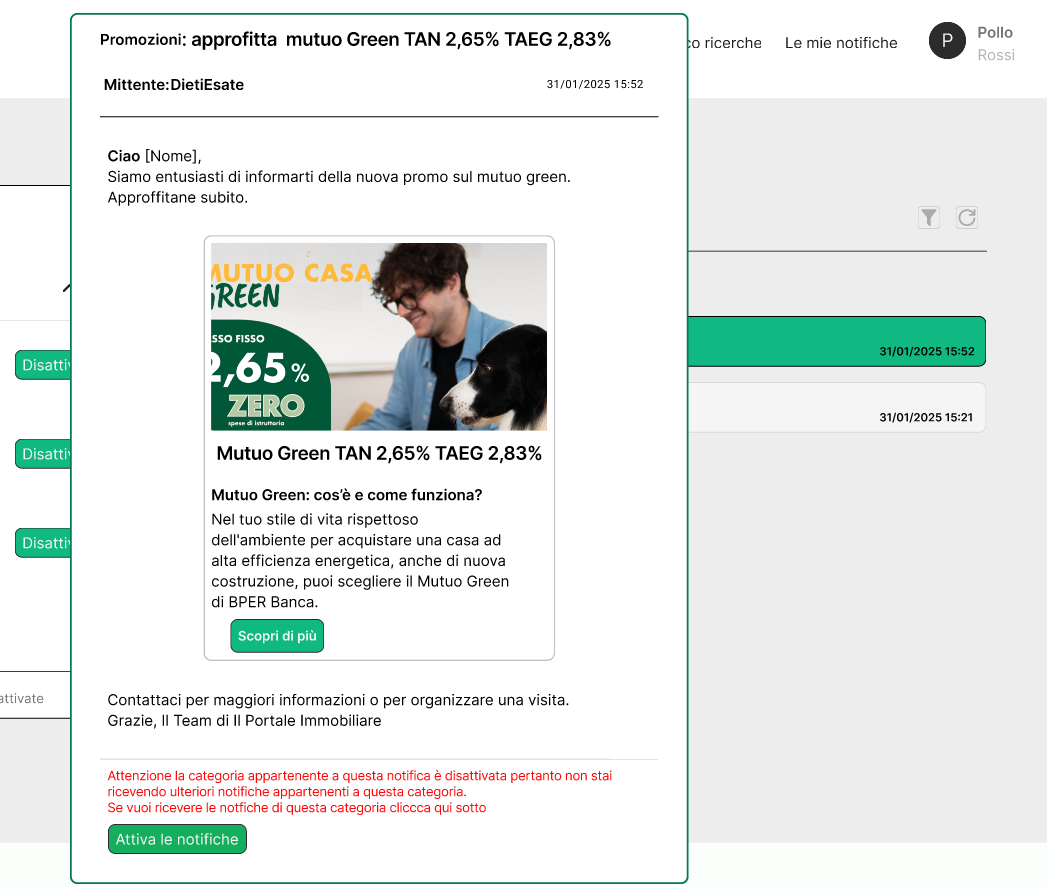
\includegraphics[width=0.4\textwidth]{Immagini/Mockup/notifiche/estensione A/disattivato.png} \\
                Cockburn: extension A.5
            \end{tabular}
        };
        
        % Disegna le frecce
        \draw[->, thick] (img1) -- (img2);
        \draw[->, thick] (img2) -- (img3);
      
    \end{tikzpicture}
    \caption{Mockup: estensione A della tabella di Cockburn del caso d'uso disattiva/attiva categoria notifica}
    \label{fig:mockup_estensione_A_disattiva_notifiche}
\end{figure}

\newpage


\clearpage
\newpage
\subsubsection{Estensione B: Ripristino di un Annuncio Precedente}
Se l’utente sceglie di \textbf{ripristinare l’annuncio precedente}, il sistema avvia un processo di caricamento per fornire un feedback visivo sulla ripresa dei dati. Sebbene i dati siano salvati localmente e il recupero sia immediato, un \textbf{indicatore di caricamento fittizio} viene mostrato per alcuni secondi prima di caricare la schermata.

Questa soluzione è basata sul principio della \textbf{coerenza con le aspettative dell’utente} \cite{shneiderman2004}. In un contesto digitale, un ripristino istantaneo potrebbe apparire innaturale e creare confusione. L’indicatore di caricamento:
\begin{itemize}
    \item Rafforza la percezione di un processo in corso, migliorando la trasparenza dell’operazione.
    \item Evita che l’utente si domandi se il recupero sia realmente avvenuto o se ci siano stati problemi tecnici.
    \item Contribuisce a una transizione più fluida tra stati dell’interfaccia.
\end{itemize}

Una volta completato il caricamento, il sistema presenta l’interfaccia con i dati precedentemente salvati, consentendo all’utente di riprendere il processo da dove era stato interrotto.


\begin{figure}[ht]
    \centering
    \begin{tikzpicture}[node distance=1.5cm and 1cm, auto]
        % Nodo per immagine 1 con didascalia sotto
        \node (img1) {
            \begin{tabular}{c}
                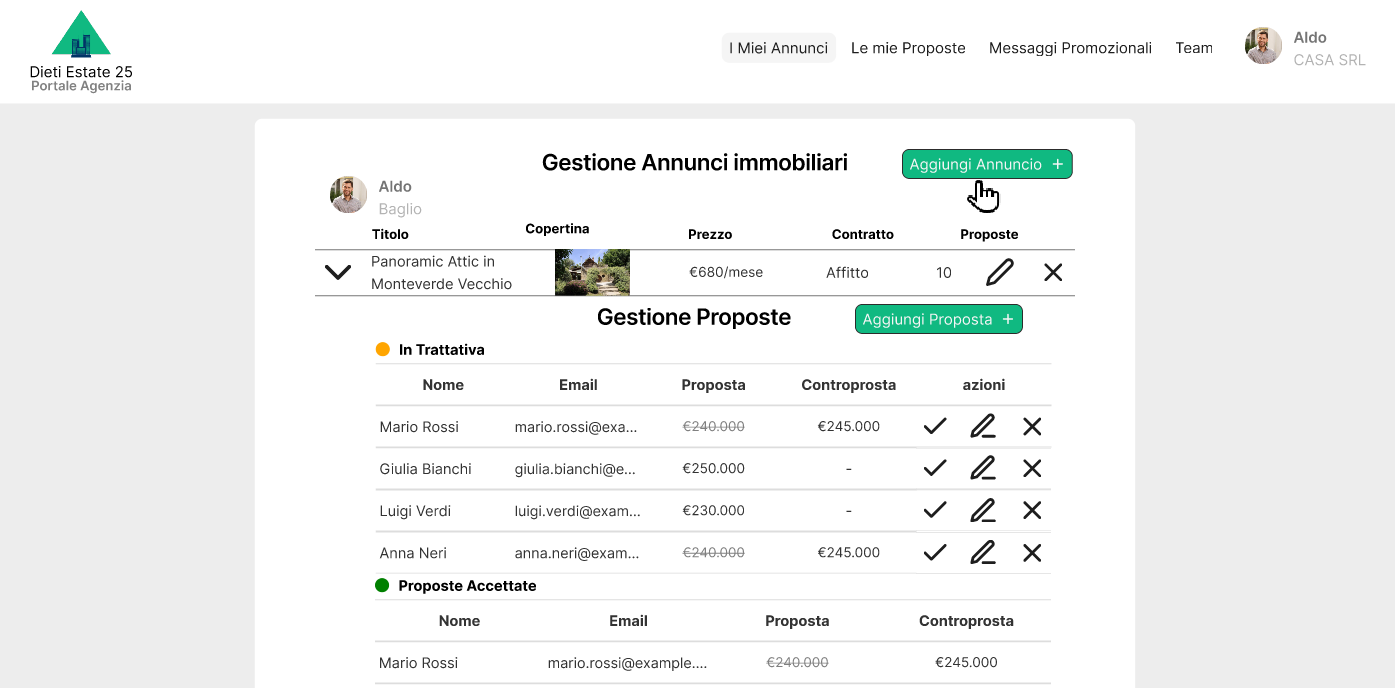
\includegraphics[width=0.7\textwidth]{Immagini/Mockup/aggiungi annuncio/estensione B/step1.png} \\
                click nuovo annuncio
            \end{tabular}
        };
        
        % Nodo per immagine 2 con didascalia sotto, posizionato a destra di img1
        \node (img2) [below=of img1] {
            \begin{tabular}{c}
                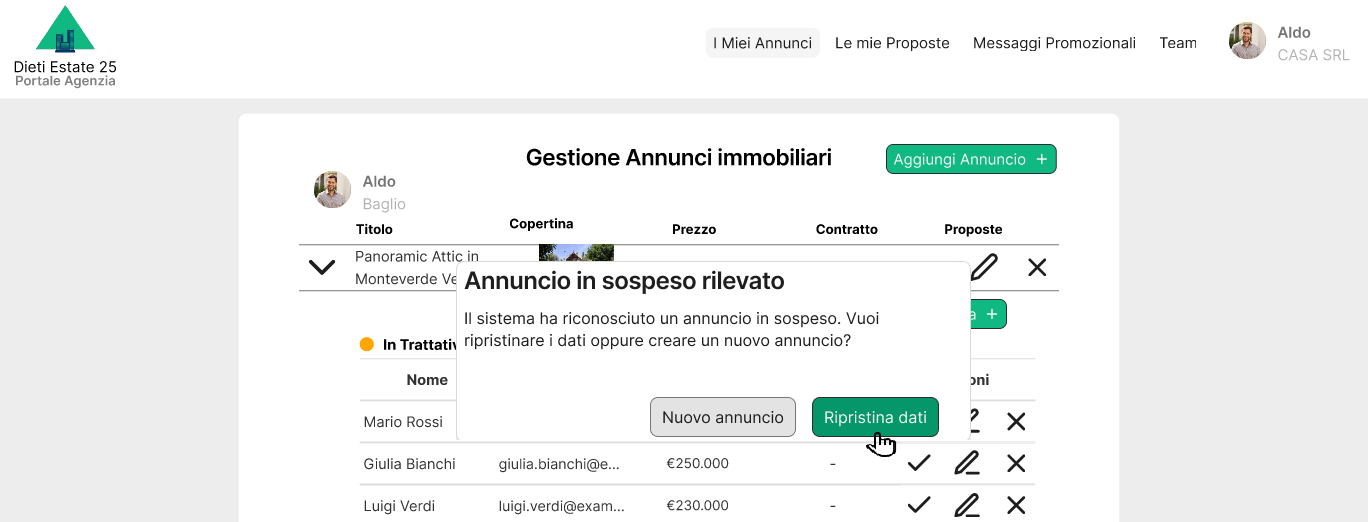
\includegraphics[width=0.7\textwidth]{Immagini/Mockup/aggiungi annuncio/estensione B/step2.png} \\
                Cockburn: extension B.2/B.3/B.4
            \end{tabular}
        };
        
        % Nodo per immagine 3 con didascalia sotto, posizionato sotto img2
        \node (img3) [below=of img2] {
            \begin{tabular}{c}
                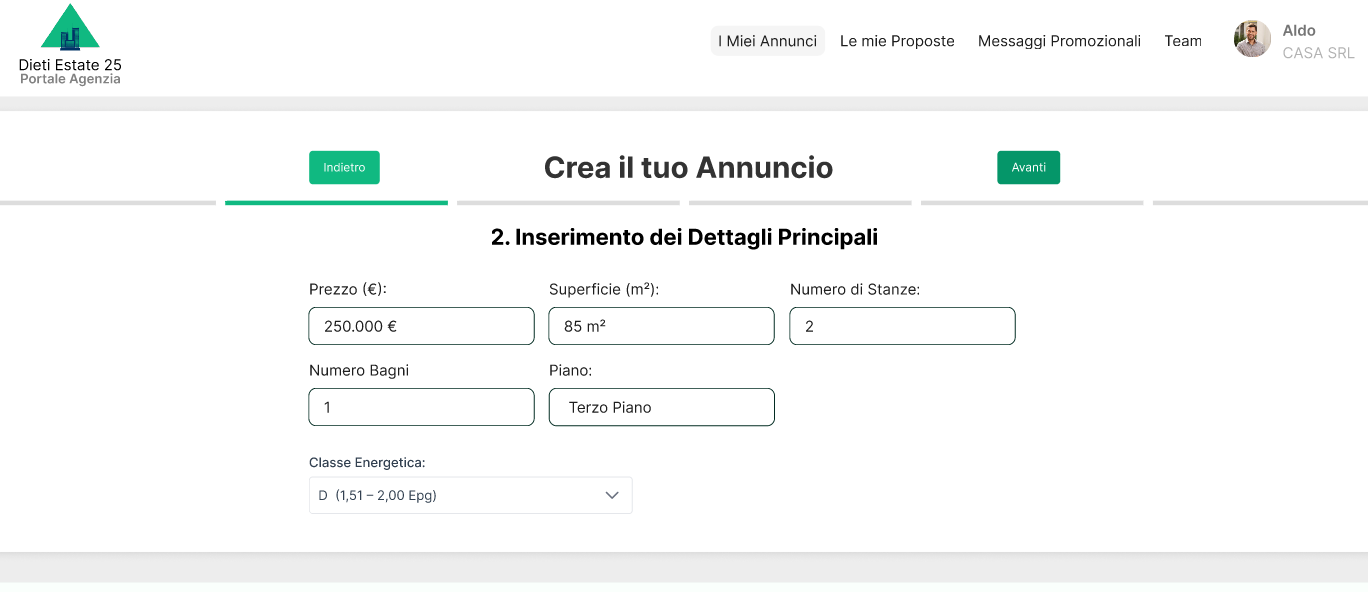
\includegraphics[width=0.7\textwidth]{Immagini/Mockup/aggiungi annuncio/estensione B/step3.png} \\
                Cockburn: extension B.5
            \end{tabular}
        };
        
        % Disegna le frecce
        \draw[->, thick] (img1) -- (img2);
        \draw[->, thick] (img2) -- (img3);
      
    \end{tikzpicture}
    \caption{Mockup: estensione B della tabella di Cockburn del caso d'uso nuovo annuncio}
    \label{fig:mockup_estensione_B_aggiungi_annuncio}
\end{figure}

\newpage



\input{Requisiti Del Software/Analisi dei Requisiti/Mockup/disattivazione notifiche/estensione c}

\clearpage
\newpage

\subsubsection{Estensione D: Modifica Rapida dello Stato delle Notifiche con Attivazione Immediata}

Questa variante rappresenta l’approccio duale dell’\textbf{Estensione C}, semplificando ulteriormente l’attivazione delle notifiche. L’obiettivo è ridurre i passaggi necessari per riattivare una categoria disattivata, mantenendo comunque un controllo chiaro sulla disattivazione.

\vspace{0.5cm}
\subsubsection{Interfaccia e Interazione}
Analogamente all’\textbf{Estensione C}, ogni categoria nella barra laterale dispone di un pulsante contestuale per modificarne lo stato. Il pulsante può assumere due stati:

\begin{itemize}
    \item \textbf{Attiva}, se la categoria è attualmente disabilitata.
    \item \textbf{Disattiva}, se la categoria è attualmente abilitata.
\end{itemize}

Le interazioni dell’utente variano a seconda dell’azione eseguita:

\begin{itemize}
    \item \textbf{Disattivazione di una categoria}:
    \begin{itemize}
        \item Al clic su \textbf{Disattiva}, appare un popup di conferma che informa l’utente sulle conseguenze della scelta, prevenendo azioni accidentali in linea con i principi di Nielsen \cite{nielsen1995}.
        \item Se confermata, la categoria viene spostata nella sezione delle notifiche disattivate tramite un’animazione di transizione.
        \item Il pulsante cambia stato, diventando \textbf{Attiva}, fornendo un feedback visivo chiaro sulla modifica.
    \end{itemize}
    
    \item \textbf{Attivazione di una categoria}:
    \begin{itemize}
        \item Al clic su \textbf{Attiva}, il sistema aggiorna immediatamente lo stato della notifica senza richiedere una conferma esplicita.
        \item La categoria viene spostata nella sezione delle notifiche attive con un’animazione fluida, applicando il principio della \textbf{gestalt della continuità} \cite{miller1956}.
        \item Il pulsante cambia stato in \textbf{Disattiva}, rendendo la modifica evidente e intuitiva.
    \end{itemize}
\end{itemize}

\subsubsection{Feedback Visivo e UX Design}
L’esperienza utente è ottimizzata tramite tecniche di design che garantiscono chiarezza e immediatezza:

\begin{itemize}
    \item \textbf{Popup di conferma per la disattivazione}: aiuta a prevenire errori e rende consapevole l’utente delle conseguenze della scelta \cite{nielsen1995}.
    \item \textbf{Animazione di transizione}: assicura una continuità visiva fluida nello spostamento delle categorie, migliorando la percezione del cambiamento \cite{miller1956}.
    \item \textbf{Aggiornamento immediato dello stato del pulsante}: il cambio di testo e colore riflette lo stato corrente della categoria, riducendo l’ambiguità e migliorando la prevedibilità dell’interazione.
\end{itemize}

Questa estensione semplifica l’attivazione delle notifiche, eliminando il passaggio della conferma e migliorando la fluidità dell’interazione, senza compromettere il controllo dell’utente sulla gestione delle proprie preferenze.

\begin{figure}[ht]
    \centering
    \begin{tikzpicture}[node distance=1.5cm and 1cm, auto]
        % Nodo per immagine 1 con didascalia sotto
        \node (img1) {
            \begin{tabular}{c}
                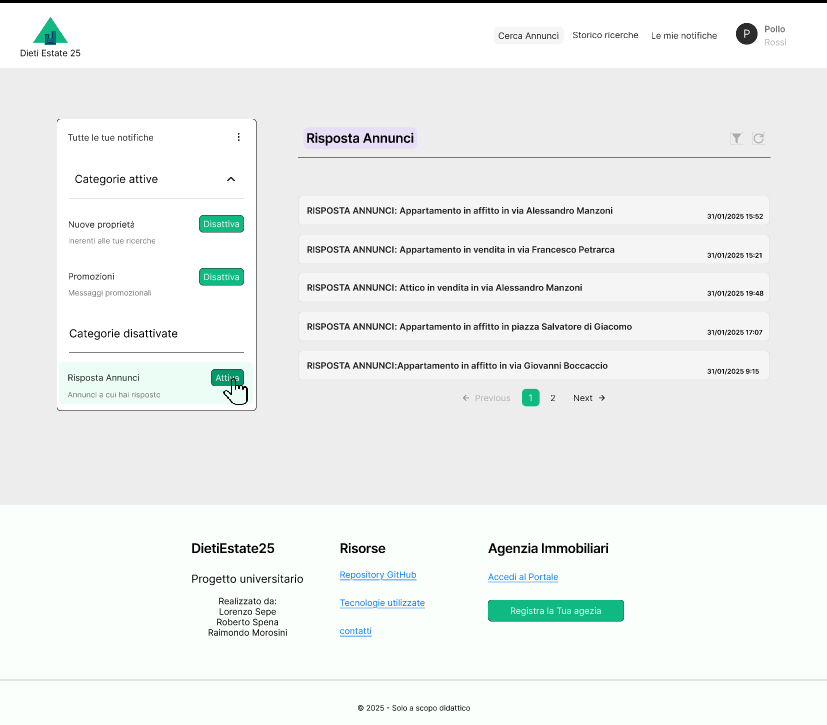
\includegraphics[width=0.6\textwidth]{Immagini/Mockup/notifiche/estensione D/clickAttiva.png} \\
                Cockburn: Extension D.2
            \end{tabular}
        };
        
        % Nodo per immagine 2 con didascalia sotto, posizionato a destra di img1
        \node (img2) [below=of img1] {
            \begin{tabular}{c}
                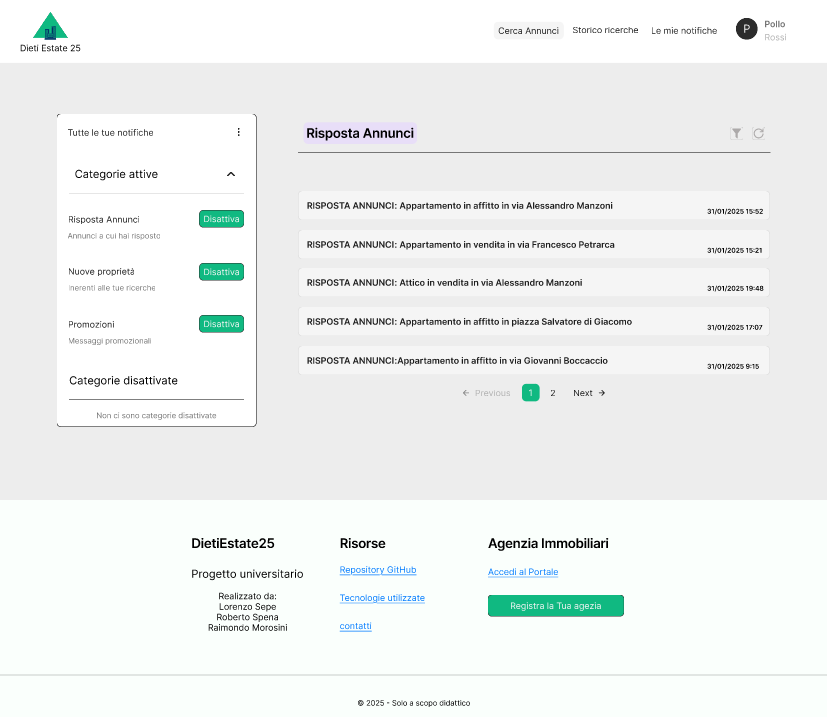
\includegraphics[width=0.6\textwidth]{Immagini/Mockup/notifiche/estensione D/attivato.png} \\
                Cockburn: step 8/9/10
            \end{tabular}
        };
        
        % Disegna le frecce
        \draw[->, thick] (img1) -- (img2);
      
    \end{tikzpicture}
    \caption{Mockup: estensione D della tabella di Cockburn del caso d'uso disattiva/attiva categoria notifica}
    \label{fig:mockup_estensione_D_disattiva_notifiche}
\end{figure}

\newpage



\clearpage
\newpage

\subsubsection{Estensione E: Errore Durante la Modifica dello Stato delle Categorie di Notifica}

Nel caso in cui si verifichi un errore durante il tentativo di modifica dello stato di una categoria di notifica, viene visualizzato un messaggio di errore sotto forma di un popup informativo. Il messaggio informa l'utente che la modifica non è riuscita e lo invita a riprovare più tardi, senza salvare le modifiche effettuate.

\vspace{0.5cm}
\subsubsection{Gestione dell'Errore e Feedback Utente} Il popup di errore presenta i seguenti elementi chiave: \begin{itemize} \item \textbf{Messaggio chiaro e informativo}: il messaggio comunica all'utente che l'operazione non è andata a buon fine, senza entrare in dettagli tecnici, per ridurre il rischio di frustrazione. L'utente viene anche informato che l'operazione non è stata completata e che le modifiche non sono state salvate. \item \textbf{Pulsante “Ok”}: consente all'utente di chiudere il popup e tornare all'interfaccia principale. Il pulsante di conferma è chiaro e consente di riprendere l'interazione senza indugi. \end{itemize}

\subsubsection{Principi di Design Applicati} L'approccio di gestione dell'errore in questa estensione si fonda sui seguenti principi di UX e usabilità: \begin{itemize} \item \textbf{Visibilità dello stato del sistema} \cite{nielsen1995}: l'errore è comunicato all'utente attraverso un popup che evidenzia chiaramente che il sistema non è riuscito a completare l'operazione. \item \textbf{Prevenzione degli errori} \cite{nielsen1995}: sebbene l'errore non possa essere evitato completamente, il sistema offre un feedback immediato e comprensibile, impedendo all'utente di rimanere confuso o incerto sullo stato dell'operazione. \item \textbf{Semplicità e chiarezza} \cite{nielsen1995}: il messaggio di errore è semplice e diretto, senza sovraccaricare l'utente con informazioni tecniche. L'invito a riprovare più tardi mantiene il flusso di lavoro semplice e lineare. \item \textbf{Controllo dell'utente} \cite{norman1988}: l'utente ha il pieno controllo sulla gestione dell'errore, poiché il popup permette di chiudere facilmente l'interfaccia e riprendere l'attività, mantenendo un'esperienza utente fluida. \end{itemize}

Questa soluzione di gestione dell'errore è progettata per garantire un'esperienza utente chiara e senza frustrazioni, minimizzando il disagio derivante da errori tecnici imprevisti e offrendo un percorso semplice per riprendere l'interazione.
\begin{figure}[ht]
    \centering
    \begin{tikzpicture}[node distance=1.5cm and 1cm, auto]
        % Nodo per immagine 1 con didascalia sotto
        \node (img1) {
            \begin{tabular}{c}
                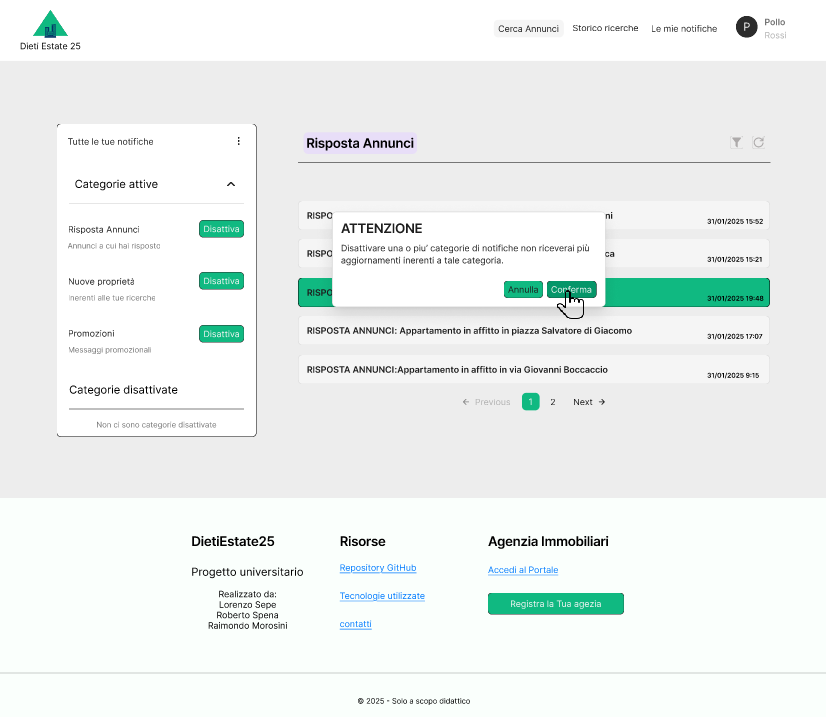
\includegraphics[width=0.6\textwidth]{Immagini/Mockup/notifiche/estensione E/click conferma.png} \\
                Cockburn: step 7
            \end{tabular}
        };
        
        % Nodo per immagine 2 con didascalia sotto, posizionato a destra di img1
        \node (img2) [below=of img1] {
            \begin{tabular}{c}
                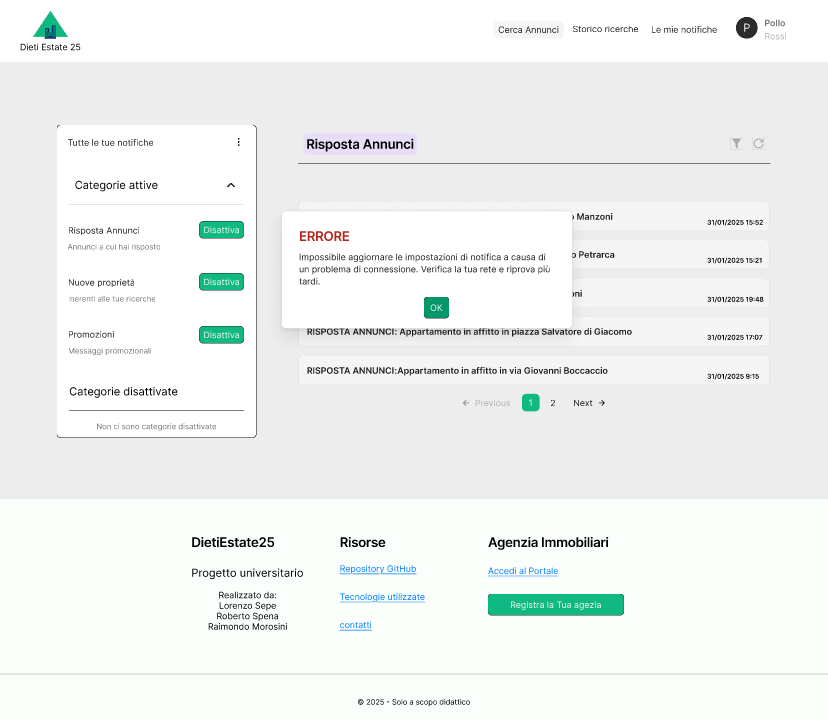
\includegraphics[width=0.6\textwidth]{Immagini/Mockup/notifiche/estensione E/errore.png} \\
                Cockburn: Extension E.7/E.8
            \end{tabular}
        };
        
        % Disegna le frecce
        \draw[->, thick] (img1) -- (img2);
      
    \end{tikzpicture}
    \caption{Mockup: estensione E della tabella di Cockburn del caso d'uso disattiva/attiva categoria notifica}
    \label{fig:tikz_flow}
\end{figure}

\newpage



\clearpage
\newpage

\subsubsection{Estensione F: Riattivazione Notifiche dalle Notifiche Disattivate}

Questa estensione consente all’utente di riattivare una categoria di notifiche direttamente da una notifica precedentemente ricevuta e appartenente a una categoria disattivata. L’obiettivo è fornire un meccanismo immediato per ripristinare le notifiche quando l’utente si rende conto della loro utilità.

\vspace{0.5cm}
\subsubsection{Indicazione dello Stato e Call-to-Action}
Quando una notifica proviene da una categoria disattivata, il sistema mostra un messaggio di avviso evidenziato che informa l’utente che non riceverà più aggiornamenti simili. Il pulsante associato cambia stato e diventa un invito all’azione con il testo “Riattiva notifiche”. Questo sfrutta il \textbf{principio della reversibilità} \cite{shneiderman2004}, permettendo all’utente di annullare la decisione precedente senza difficoltà.

\vspace{0.5cm}
\subsubsection{Feedback Visivo e Conferma della Riattivazione}
Alla pressione del pulsante, il testo cambia colore in verde e il messaggio informativo si aggiorna, confermando che le notifiche per quella categoria sono state riattivate. Il sistema può fornire un’ulteriore conferma con un breve messaggio di notifica o una vibrazione del dispositivo per enfatizzare l’azione completata.

\vspace{0.5cm}
\subsubsection{Coerenza con il Modello di Gestione Notifiche}
Questa estensione rafforza la coerenza dell’interfaccia di gestione delle notifiche, mantenendo le scelte dell’utente sempre modificabili e promuovendo un’interazione trasparente e prevedibile. L’utente può così gestire le notifiche senza dover accedere necessariamente alla schermata delle impostazioni, riducendo il carico cognitivo e migliorando l’usabilità complessiva del sistema.\begin{figure}[ht]
    \centering
    \begin{tikzpicture}[node distance=1.5cm and 1cm, auto]
        % Nodo per immagine 1 con didascalia sotto
        \node (img1) {
            \begin{tabular}{c}
                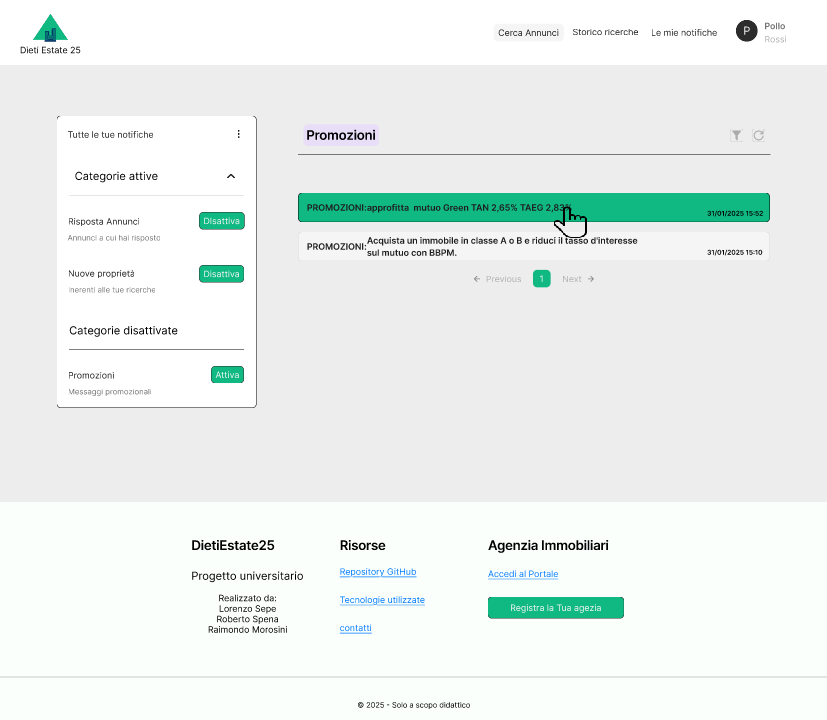
\includegraphics[width=0.4\textwidth]{Immagini/Mockup/notifiche/estensione F/clickNotifica.png} \\
                Cockburn: Extension F.2
            \end{tabular}
        };
        
        % Nodo per immagine 2 con didascalia sotto, posizionato a destra di img1
        \node (img2) [below=of img1] {
            \begin{tabular}{c}
                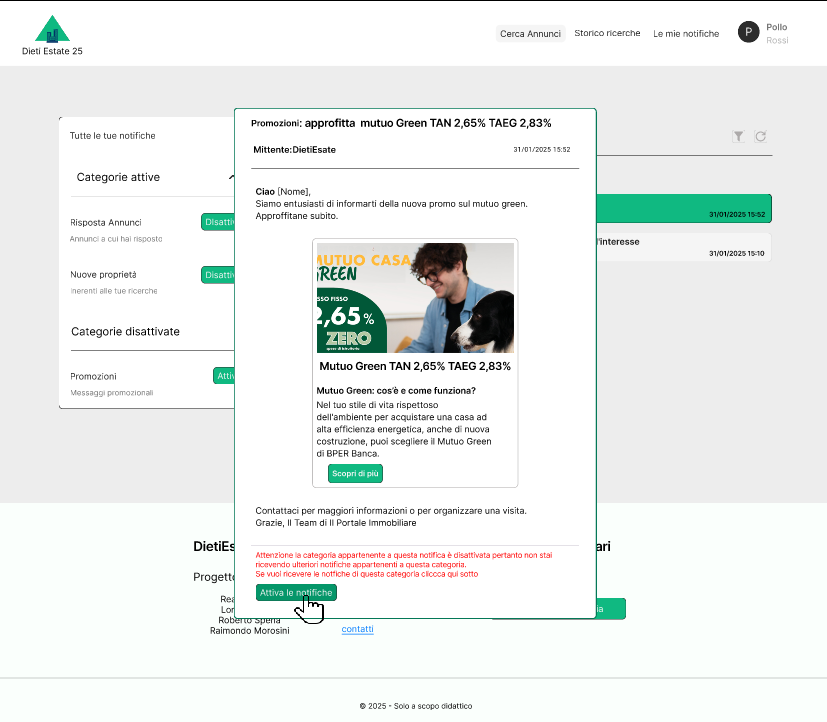
\includegraphics[width=0.4\textwidth]{Immagini/Mockup/notifiche/estensione F/clickAttiva.png} \\
                Cockburn: Extension F.3
            \end{tabular}
        };
        
        % Nodo per immagine 3 con didascalia sotto, posizionato sotto img2
        \node (img3) [below=of img2] {
            \begin{tabular}{c}
                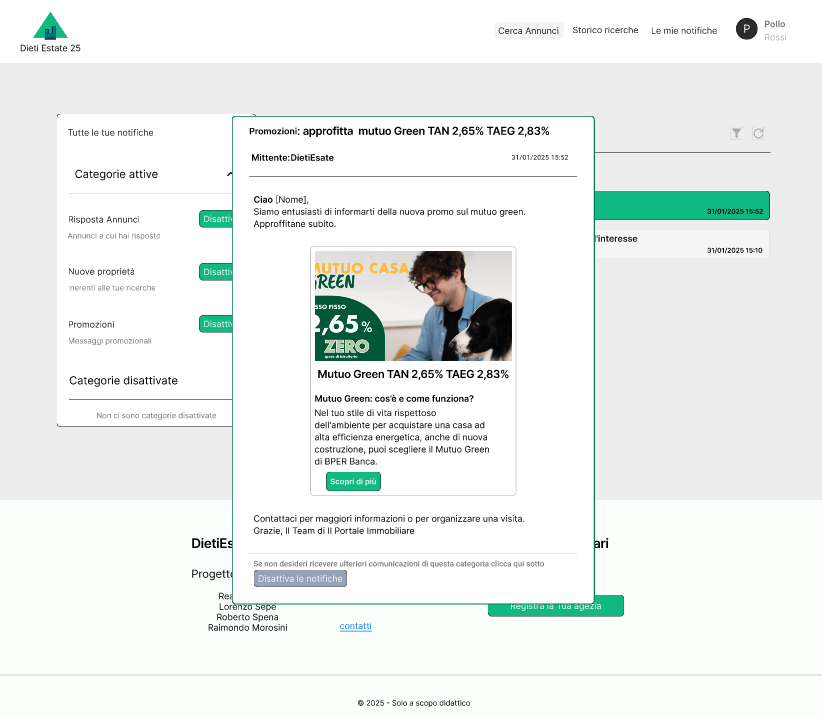
\includegraphics[width=0.4\textwidth]{Immagini/Mockup/notifiche/estensione F/attivato.png} \\
                Cockburn: Extension F.4/F.5
            \end{tabular}
        };
        
        % Disegna le frecce
        \draw[->, thick] (img1) -- (img2);
        \draw[->, thick] (img2) -- (img3);
      
    \end{tikzpicture}
    \caption{Mockup: estensione F della tabella di Cockburn del caso d'uso disattiva/attiva categoria notifica}
    \label{fig:mockup_estensione_F_disattiva_notifiche}
\end{figure}

\newpage



\clearpage
\newpage

La \textbf{valutazione dell'usabilità} rappresenta una fase essenziale nel processo di sviluppo di un’interfaccia utente, consentendo di valutare l'efficacia, l’efficienza e la soddisfazione dell’utente nell’interazione con il sistema. In particolare, l'uso di mockup interattivi offre la possibilità di raccogliere feedback sulle scelte di design prima ancora della fase di sviluppo, riducendo i costi di eventuali revisioni e migliorando la qualità dell’esperienza utente.
\newline
L'obiettivo principale di questa sezione è identificare eventuali problemi di navigazione, ambiguità nelle interazioni o difficoltà nella comprensione delle funzionalità, al fine di ottimizzare l'interfaccia prima del rilascio definitivo.

\section{Expert Reviews / Inspections}

Per valutare la qualità complessiva dell’esperienza utente e la coerenza progettuale del sistema, è stata pianificata una revisione sistematica dell’interfaccia basata su una \textbf{valutazione euristica} secondo i principi di Nielsen \cite{nielsen1995}.  
L’attività ha avuto l’obiettivo di identificare punti di forza, criticità e incoerenze nel design, analizzando in due fasi distinte il \textit{prototipo realizzato in Figma} e successivamente la \textit{versione web implementata}.  

La revisione del prototipo Figma ha rappresentato un passaggio fondamentale prima dello sviluppo effettivo: ha consentito di riflettere in modo critico sulle scelte di interfaccia, di validare le principali logiche di navigazione e di anticipare eventuali problemi di usabilità.  
A differenza della versione web, il prototipo non consente un’interazione reale, ma offre comunque una base solida per verificare la chiarezza dei flussi e la coerenza visiva complessiva.

\subsection*{Obiettivi della Review}

Gli obiettivi principali dell’attività di \textit{Expert Review} sono stati:
\begin{itemize}
    \item Valutare la \textbf{usabilità} dei flussi principali del sistema, verificando la chiarezza dei percorsi e delle azioni disponibili.
    \item Analizzare la \textbf{coerenza visiva} rispetto alle linee guida di design definite nel brand e nel prototipo.
    \item Individuare problemi di \textbf{chiarezza, navigabilità e feedback} che possano compromettere l’esperienza d’uso.
    \item Identificare eventuali mancanze o ridondanze, con l’obiettivo di \textbf{migliorare la struttura informativa e la consistenza visiva}.
    \item Definire raccomandazioni per le fasi successive di sviluppo, in vista della revisione della \textbf{versione web funzionante}.
\end{itemize}

\subsection*{Motivazione della Checklist Scelta}

Per garantire una valutazione sistematica, replicabile e comparabile tra diverse aree dell’interfaccia, è stata utilizzata una \textbf{checklist di usabilità} costruita sui dieci principi di Nielsen.  
Questo approccio è stato scelto perché:
\begin{itemize}
    \item consente una \textbf{autovalutazione strutturata} anche in assenza di utenti reali o revisori esterni;
    \item può essere applicato sia a \textbf{prototipi statici} (come quelli sviluppati in Figma) sia a \textbf{interfacce interattive} e funzionanti;
    \item copre in modo ampio le dimensioni fondamentali dell’usabilità: visibilità dello stato del sistema, coerenza, prevenzione degli errori, efficienza, chiarezza e supporto all’utente.
\end{itemize}

\subsection*{Struttura della Checklist Euristica}

La checklist adottata si basa sui dieci principi classici di Nielsen, riformulati in forma di domande operative per adattarli al contesto del progetto.  
Ogni criterio è stato utilizzato come base per analizzare il prototipo Figma e successivamente la versione web.

\begin{table}[H]
\centering
\begin{tabular}{p{0.7cm} p{4cm} p{8cm}}
\hline
\textbf{\#} & \textbf{Criterio} & \textbf{Domanda di verifica} \\
\hline
1 & Visibilità dello stato del sistema & L’utente riceve sempre un feedback visivo o testuale dopo un’azione (salvataggio, invio, errore)? \\
2 & Corrispondenza tra sistema e mondo reale & Terminologia, icone e messaggi sono coerenti con il linguaggio del dominio immobiliare? \\
3 & Controllo e libertà dell’utente & È possibile annullare o correggere facilmente un’azione? \\
4 & Coerenza e standard & Colori, stili e componenti rispettano il design definito nel brand e nel prototipo? \\
5 & Prevenzione e gestione degli errori & I form prevengono gli errori tramite validazioni e messaggi chiari? \\
6 & Efficienza e flessibilità d’uso & Le operazioni più frequenti possono essere eseguite rapidamente, anche da dispositivi mobili? \\
7 & Chiarezza del contenuto & Testi e etichette sono comprensibili e privi di ambiguità? \\
8 & Supporto al riconoscimento & Le opzioni principali sono visibili e non richiedono memoria a breve termine all’utente? \\
9 & Feedback e conferme & Sono presenti messaggi di conferma dopo azioni critiche (pubblicazione, eliminazione, invio)? \\
10 & Aiuto e documentazione & È disponibile un supporto o una guida per l’utente in caso di difficoltà? \\
\hline
\end{tabular}
\caption{Checklist di valutazione euristica basata sui principi di Nielsen.}
\end{table}

\bigskip

La sezione seguente presenta nel dettaglio l’applicazione di questa checklist al \textbf{prototipo Figma}, con un’analisi critica dei dieci criteri e una successiva autovalutazione sintetica dei risultati ottenuti.

\subsection{Expert Review sul Prototipo Figma}

L’attività di revisione euristica è stata condotta sul prototipo sviluppato in \textit{Figma} prima della realizzazione della versione web.  
L’obiettivo è stato valutare il livello di usabilità e coerenza delle principali interfacce progettate, verificando la presenza di feedback, la chiarezza dei flussi e la consistenza grafica secondo i dieci principi di Nielsen.  

\subsubsection*{1. Visibilità dello stato del sistema}  
Nel prototipo sono stati previsti diversi meccanismi di feedback.  
Nei flussi \textit{Fai controproposta} e \textit{Registra dipendente} sono stati inseriti \textbf{indicatori di caricamento} per mostrare lo stato del sistema durante le operazioni.  
In tutti i form è presente un \textbf{sistema di validazione immediata}: i campi non validi vengono evidenziati in rosso e, nel caso della \textit{creazione di un annuncio}, il processo è suddiviso in step.  
Quando uno step contiene errori, il suo indicatore cambia colore e un box iniziale riepiloga i campi non validi.  
Tutti i flussi analizzati includono un \textbf{doppio messaggio di conferma} prima dell’esecuzione definitiva, ad eccezione della creazione di un annuncio.  
Nel complesso, il prototipo offre una buona visibilità dello stato del sistema, con l’unica criticità relativa all’assenza di conferma dopo la pubblicazione.

\subsubsection*{2. Corrispondenza tra sistema e mondo reale}  
Il linguaggio utilizzato è \textbf{semplice e diretto}, adatto agli utenti finali.  
Le sezioni con terminologia più specifica (legate alle agenzie immobiliari) risultano coerenti con il dominio e adatte a un pubblico professionale.  
Sono state impiegate \textbf{icone standard e universalmente riconoscibili}, affiancate da \textbf{tooltip descrittivi} che ne chiariscono il significato.  
L’unico aspetto ancora da migliorare riguarda la \textbf{scelta delle icone nello stepper} di creazione annuncio, dove sarebbe utile uno studio mirato per rendere più intuitivi i passaggi.

\subsubsection*{3. Controllo e libertà dell’utente}  
Il prototipo garantisce buone possibilità di annullamento e controllo.  
Tutti i popup includono una \textbf{“X” per chiudere o annullare}, e i messaggi di conferma prevedono esplicitamente un pulsante \textit{Annulla}.  
Le azioni potenzialmente distruttive, come la \textbf{disattivazione delle notifiche}, richiedono conferma; viceversa, l’attivazione non la richiede poiché non comporta rischi di perdita di dati.  
La progettazione su questo punto è stata ritenuta soddisfacente e coerente con le aspettative di usabilità.

\subsubsection*{4. Coerenza e standard}  
Il design mantiene nel complesso una \textbf{coerenza visiva} nei colori e nello stile dei pulsanti, in linea con il concept minimalista del progetto.  
Tuttavia, si è rilevata una \textbf{mancanza di uniformità nei popup}: nei diversi casi d’uso sono stati utilizzati modelli leggermente differenti, frutto di sperimentazioni grafiche ancora non consolidate.  
In fase di sviluppo sarà necessario \textbf{uniformare componenti e modali}, garantendo una coerenza piena tra tutti i flussi.

\subsubsection*{5. Prevenzione e gestione degli errori}  
La prevenzione degli errori è uno degli aspetti più curati nel prototipo.  
I form mostrano in tempo reale i campi non validi e forniscono \textbf{indicazioni visive chiare (rosso)} insieme a messaggi testuali.  
La combinazione di validazione immediata e conferme d’azione riduce significativamente il rischio di errori da parte dell’utente.  
Questo punto risulta pienamente soddisfatto.

\subsubsection*{6. Efficienza e flessibilità d’uso}  
Essendo un prototipo statico, l’efficienza d’uso è valutabile solo in parte.  
L’interfaccia è stata progettata per un utilizzo anche da \textbf{dispositivi verticali}, ma la resa migliore si ottiene in \textbf{orientamento orizzontale (landscape)}.  
Non sono state ancora considerate \textbf{scorciatoie o funzionalità avanzate} per utenti esperti (es. salvataggio bozza, importazione di dati da file), che potrebbero rappresentare un’evoluzione futura del progetto.  
Si riconosce quindi questo come un punto da sviluppare ulteriormente.

\subsubsection*{7. Chiarezza del contenuto}  
I testi sono \textbf{brevi, diretti e privi di tecnicismi}, con un linguaggio coerente e immediato.  
Quando una sola etichetta non è sufficiente, è previsto l’uso di \textbf{tooltip esplicativi}.  
Questo approccio consente una buona comprensione del flusso anche senza documentazione aggiuntiva.

\subsubsection*{8. Supporto al riconoscimento}  
Le principali funzioni sono \textbf{raggiungibili in pochi clic}.  
La \textit{header bar} consente di passare rapidamente tra ricerca, storico annunci e notifiche; inoltre, il passaggio tra l’area cliente e quella agenzia è reso accessibile dal \textit{footer}.  
Un test di eye-tracking condotto su alcune schermate del prototipo ha confermato la \textbf{corretta collocazione visiva} degli elementi più rilevanti, validando l’efficacia della struttura.

\subsubsection*{9. Feedback e conferme}  
Le operazioni critiche, come eliminazione o modifica, utilizzano lo stesso colore principale del sito, il che può generare confusione con azioni neutre.  
Si suggerisce di differenziare \textbf{visivamente le azioni distruttive} (es. usando toni di rosso o arancione) e di inserire messaggi di conferma più evidenti per i processi più delicati.  
Nonostante ciò, il comportamento rimane accettabile per utenti esperti.

\subsubsection*{10. Aiuto e documentazione}  
Non è stato previsto un sistema di aiuto, documentazione o FAQ, poiché il prototipo nasce in un contesto accademico.  
Tuttavia, in una versione completa sarebbe opportuno introdurre:  
\begin{itemize}
    \item una \textbf{sezione FAQ} o assistenza per i problemi più comuni;  
    \item \textbf{overlay o onboarding guidato} per i nuovi utenti;  
    \item pulsanti contestuali “Come funziona” nelle pagine più complesse.  
\end{itemize}

\subsubsection*{Autovalutazione e sintesi}  
La tabella seguente riassume il livello di soddisfacimento delle euristiche sul prototipo Figma (0 = non soddisfatto, 1 = parzialmente soddisfatto, 2 = soddisfatto).

\begin{table}[h!]
\centering
\begin{tabular}{p{0.4cm} p{4cm} p{1.5cm} p{7cm}}
\hline
\textbf{\#} & \textbf{Criterio} & \textbf{Valutazione} & \textbf{Motivazione sintetica} \\ \hline
1 & Visibilità stato & 2 & Feedback e validazioni chiare, manca solo conferma finale in creazione annuncio \\
2 & Corrispondenza mondo reale & 2 & Linguaggio semplice e coerente, icone chiare \\
3 & Controllo e libertà & 2 & Annulla e conferme sempre presenti \\
4 & Coerenza e standard & 1 & Popup non uniformi tra i flussi \\
5 & Prevenzione errori & 2 & Validazione in tempo reale e segnalazioni visive \\
6 & Efficienza/flessibilità & 1 & Assenza di scorciatoie e ottimizzazione solo parziale per mobile \\
7 & Chiarezza del contenuto & 2 & Testi sintetici e coerenti \\
8 & Supporto al riconoscimento & 2 & Navigazione semplice e confermata da test visivi \\
9 & Feedback/Conferme & 1 & Colori azioni critiche da differenziare \\
10 & Aiuto/Documentazione & 0 & Non prevista sezione di supporto \\ \hline
\end{tabular}
\caption{Autovalutazione euristica del prototipo Figma secondo i principi di Nielsen.}
\end{table}

\subsubsection*{Conclusioni}  
Il prototipo Figma risulta \textbf{completo, coerente e ben strutturato}, con una gestione accurata dei form, validazioni efficaci e buona leggibilità generale.  
I principali margini di miglioramento riguardano la \textbf{coerenza visiva dei popup}, la \textbf{differenziazione dei feedback critici} e l’assenza di un \textbf{sistema di aiuto} o onboarding.  
Questi aspetti costituiranno la base per le iterazioni successive e per l’ottimizzazione della versione web finale.



TODO Da fare bene la seocnda parte 

\textbf{Versione Web:} la checklist è stata applicata all’intero insieme di requisiti e funzionalità richiesti dal docente, permettendo una valutazione completa dell’interfaccia e dei flussi principali del sistema.

\subsection*{Definizione della Checklist di Usabilità}

La checklist elaborata si basa su una selezione adattata delle euristiche di Nielsen, ridotte e riformulate per meglio aderire al contesto del progetto.  
Ogni criterio è espresso come domanda di verifica utilizzata per valutare sia il prototipo sia il sito web.

\begin{table}[h!]
\centering
\begin{tabular}{p{0.8cm} p{4cm} p{7cm}}
\hline
\textbf{\#} & \textbf{Criterio} & \textbf{Domanda di verifica} \\
\hline
1 & Visibilità dello stato del sistema & L’utente riceve sempre un feedback visivo o testuale in seguito a un’azione (es. salvataggio, invio, errore)? \\
2 & Corrispondenza tra sistema e mondo reale & Terminologia, icone e messaggi sono coerenti con il linguaggio del dominio immobiliare? \\
3 & Controllo e libertà dell’utente & È possibile annullare o correggere facilmente un’azione (es. modifica o cancellazione di un annuncio)? \\
4 & Coerenza e standard & Colori, stili e pulsanti rispettano il design definito nel brand e nel prototipo Figma? \\
5 & Prevenzione e gestione degli errori & I form prevengono errori tramite validazioni e messaggi chiari? \\
6 & Efficienza e flessibilità d’uso & Le operazioni più frequenti possono essere completate rapidamente e da dispositivi mobili verticali? \\
7 & Chiarezza del contenuto & I testi e le etichette guidano l’utente nel flusso, senza ambiguità? \\
8 & Supporto al riconoscimento & Le opzioni principali sono sempre visibili senza richiedere memoria a breve termine all’utente? \\
9 & Feedback e conferme & Sono presenti messaggi di conferma dopo operazioni critiche (es. pubblicazione, eliminazione, invio)? \\
10 & Aiuto e documentazione & È disponibile una sezione informativa o un supporto base per l’utente? \\
\hline
\end{tabular}
\caption{Checklist di usabilità basata sulle euristiche di Nielsen, adattata al contesto del sito immobiliare multi-agenzia.}
\label{tab:checklist_usabilita}
\end{table}

\subsection*{Applicazione della Checklist}

La review è stata eseguita individualmente per ciascun caso d’uso su Figma e per l’intero insieme di funzionalità sulla versione web.  
I risultati sono stati successivamente confrontati per identificare le criticità più significative e le aree di miglioramento.




\section{Expert Reviews / Inspections}

Per valutare la qualità complessiva dell’esperienza utente e la coerenza progettuale del sistema, è stata pianificata una revisione sistematica dell’interfaccia basata su una \textbf{valutazione euristica} secondo i principi di Nielsen \cite{nielsen1995}.  
L’attività ha avuto l’obiettivo di identificare punti di forza, criticità e incoerenze nel design, analizzando in due fasi distinte il \textit{prototipo realizzato in Figma} e successivamente la \textit{versione web implementata}.  

La revisione del prototipo Figma ha rappresentato un passaggio fondamentale prima dello sviluppo effettivo: ha consentito di riflettere in modo critico sulle scelte di interfaccia, di validare le principali logiche di navigazione e di anticipare eventuali problemi di usabilità.  
A differenza della versione web, il prototipo non consente un’interazione reale, ma offre comunque una base solida per verificare la chiarezza dei flussi e la coerenza visiva complessiva.

\subsection*{Obiettivi della Review}

Gli obiettivi principali dell’attività di \textit{Expert Review} sono stati:
\begin{itemize}
    \item Valutare la \textbf{usabilità} dei flussi principali del sistema, verificando la chiarezza dei percorsi e delle azioni disponibili.
    \item Analizzare la \textbf{coerenza visiva} rispetto alle linee guida di design definite nel brand e nel prototipo.
    \item Individuare problemi di \textbf{chiarezza, navigabilità e feedback} che possano compromettere l’esperienza d’uso.
    \item Identificare eventuali mancanze o ridondanze, con l’obiettivo di \textbf{migliorare la struttura informativa e la consistenza visiva}.
    \item Definire raccomandazioni per le fasi successive di sviluppo, in vista della revisione della \textbf{versione web funzionante}.
\end{itemize}

\subsection*{Motivazione della Checklist Scelta}

Per garantire una valutazione sistematica, replicabile e comparabile tra diverse aree dell’interfaccia, è stata utilizzata una \textbf{checklist di usabilità} costruita sui dieci principi di Nielsen.  
Questo approccio è stato scelto perché:
\begin{itemize}
    \item consente una \textbf{autovalutazione strutturata} anche in assenza di utenti reali o revisori esterni;
    \item può essere applicato sia a \textbf{prototipi statici} (come quelli sviluppati in Figma) sia a \textbf{interfacce interattive} e funzionanti;
    \item copre in modo ampio le dimensioni fondamentali dell’usabilità: visibilità dello stato del sistema, coerenza, prevenzione degli errori, efficienza, chiarezza e supporto all’utente.
\end{itemize}

\subsection*{Struttura della Checklist Euristica}

La checklist adottata si basa sui dieci principi classici di Nielsen, riformulati in forma di domande operative per adattarli al contesto del progetto.  
Ogni criterio è stato utilizzato come base per analizzare il prototipo Figma e successivamente la versione web.

\begin{table}[H]
\centering
\begin{tabular}{p{0.7cm} p{4cm} p{8cm}}
\hline
\textbf{\#} & \textbf{Criterio} & \textbf{Domanda di verifica} \\
\hline
1 & Visibilità dello stato del sistema & L’utente riceve sempre un feedback visivo o testuale dopo un’azione (salvataggio, invio, errore)? \\
2 & Corrispondenza tra sistema e mondo reale & Terminologia, icone e messaggi sono coerenti con il linguaggio del dominio immobiliare? \\
3 & Controllo e libertà dell’utente & È possibile annullare o correggere facilmente un’azione? \\
4 & Coerenza e standard & Colori, stili e componenti rispettano il design definito nel brand e nel prototipo? \\
5 & Prevenzione e gestione degli errori & I form prevengono gli errori tramite validazioni e messaggi chiari? \\
6 & Efficienza e flessibilità d’uso & Le operazioni più frequenti possono essere eseguite rapidamente, anche da dispositivi mobili? \\
7 & Chiarezza del contenuto & Testi e etichette sono comprensibili e privi di ambiguità? \\
8 & Supporto al riconoscimento & Le opzioni principali sono visibili e non richiedono memoria a breve termine all’utente? \\
9 & Feedback e conferme & Sono presenti messaggi di conferma dopo azioni critiche (pubblicazione, eliminazione, invio)? \\
10 & Aiuto e documentazione & È disponibile un supporto o una guida per l’utente in caso di difficoltà? \\
\hline
\end{tabular}
\caption{Checklist di valutazione euristica basata sui principi di Nielsen.}
\end{table}

\bigskip

La sezione seguente presenta nel dettaglio l’applicazione di questa checklist al \textbf{prototipo Figma}, con un’analisi critica dei dieci criteri e una successiva autovalutazione sintetica dei risultati ottenuti.

\subsection{Expert Review sul Prototipo Figma}

L’attività di revisione euristica è stata condotta sul prototipo sviluppato in \textit{Figma} prima della realizzazione della versione web.  
L’obiettivo è stato valutare il livello di usabilità e coerenza delle principali interfacce progettate, verificando la presenza di feedback, la chiarezza dei flussi e la consistenza grafica secondo i dieci principi di Nielsen.  

\subsubsection*{1. Visibilità dello stato del sistema}  
Nel prototipo sono stati previsti diversi meccanismi di feedback.  
Nei flussi \textit{Fai controproposta} e \textit{Registra dipendente} sono stati inseriti \textbf{indicatori di caricamento} per mostrare lo stato del sistema durante le operazioni.  
In tutti i form è presente un \textbf{sistema di validazione immediata}: i campi non validi vengono evidenziati in rosso e, nel caso della \textit{creazione di un annuncio}, il processo è suddiviso in step.  
Quando uno step contiene errori, il suo indicatore cambia colore e un box iniziale riepiloga i campi non validi.  
Tutti i flussi analizzati includono un \textbf{doppio messaggio di conferma} prima dell’esecuzione definitiva, ad eccezione della creazione di un annuncio.  
Nel complesso, il prototipo offre una buona visibilità dello stato del sistema, con l’unica criticità relativa all’assenza di conferma dopo la pubblicazione.

\subsubsection*{2. Corrispondenza tra sistema e mondo reale}  
Il linguaggio utilizzato è \textbf{semplice e diretto}, adatto agli utenti finali.  
Le sezioni con terminologia più specifica (legate alle agenzie immobiliari) risultano coerenti con il dominio e adatte a un pubblico professionale.  
Sono state impiegate \textbf{icone standard e universalmente riconoscibili}, affiancate da \textbf{tooltip descrittivi} che ne chiariscono il significato.  
L’unico aspetto ancora da migliorare riguarda la \textbf{scelta delle icone nello stepper} di creazione annuncio, dove sarebbe utile uno studio mirato per rendere più intuitivi i passaggi.

\subsubsection*{3. Controllo e libertà dell’utente}  
Il prototipo garantisce buone possibilità di annullamento e controllo.  
Tutti i popup includono una \textbf{“X” per chiudere o annullare}, e i messaggi di conferma prevedono esplicitamente un pulsante \textit{Annulla}.  
Le azioni potenzialmente distruttive, come la \textbf{disattivazione delle notifiche}, richiedono conferma; viceversa, l’attivazione non la richiede poiché non comporta rischi di perdita di dati.  
La progettazione su questo punto è stata ritenuta soddisfacente e coerente con le aspettative di usabilità.

\subsubsection*{4. Coerenza e standard}  
Il design mantiene nel complesso una \textbf{coerenza visiva} nei colori e nello stile dei pulsanti, in linea con il concept minimalista del progetto.  
Tuttavia, si è rilevata una \textbf{mancanza di uniformità nei popup}: nei diversi casi d’uso sono stati utilizzati modelli leggermente differenti, frutto di sperimentazioni grafiche ancora non consolidate.  
In fase di sviluppo sarà necessario \textbf{uniformare componenti e modali}, garantendo una coerenza piena tra tutti i flussi.

\subsubsection*{5. Prevenzione e gestione degli errori}  
La prevenzione degli errori è uno degli aspetti più curati nel prototipo.  
I form mostrano in tempo reale i campi non validi e forniscono \textbf{indicazioni visive chiare (rosso)} insieme a messaggi testuali.  
La combinazione di validazione immediata e conferme d’azione riduce significativamente il rischio di errori da parte dell’utente.  
Questo punto risulta pienamente soddisfatto.

\subsubsection*{6. Efficienza e flessibilità d’uso}  
Essendo un prototipo statico, l’efficienza d’uso è valutabile solo in parte.  
L’interfaccia è stata progettata per un utilizzo anche da \textbf{dispositivi verticali}, ma la resa migliore si ottiene in \textbf{orientamento orizzontale (landscape)}.  
Non sono state ancora considerate \textbf{scorciatoie o funzionalità avanzate} per utenti esperti (es. salvataggio bozza, importazione di dati da file), che potrebbero rappresentare un’evoluzione futura del progetto.  
Si riconosce quindi questo come un punto da sviluppare ulteriormente.

\subsubsection*{7. Chiarezza del contenuto}  
I testi sono \textbf{brevi, diretti e privi di tecnicismi}, con un linguaggio coerente e immediato.  
Quando una sola etichetta non è sufficiente, è previsto l’uso di \textbf{tooltip esplicativi}.  
Questo approccio consente una buona comprensione del flusso anche senza documentazione aggiuntiva.

\subsubsection*{8. Supporto al riconoscimento}  
Le principali funzioni sono \textbf{raggiungibili in pochi clic}.  
La \textit{header bar} consente di passare rapidamente tra ricerca, storico annunci e notifiche; inoltre, il passaggio tra l’area cliente e quella agenzia è reso accessibile dal \textit{footer}.  
Un test di eye-tracking condotto su alcune schermate del prototipo ha confermato la \textbf{corretta collocazione visiva} degli elementi più rilevanti, validando l’efficacia della struttura.

\subsubsection*{9. Feedback e conferme}  
Le operazioni critiche, come eliminazione o modifica, utilizzano lo stesso colore principale del sito, il che può generare confusione con azioni neutre.  
Si suggerisce di differenziare \textbf{visivamente le azioni distruttive} (es. usando toni di rosso o arancione) e di inserire messaggi di conferma più evidenti per i processi più delicati.  
Nonostante ciò, il comportamento rimane accettabile per utenti esperti.

\subsubsection*{10. Aiuto e documentazione}  
Non è stato previsto un sistema di aiuto, documentazione o FAQ, poiché il prototipo nasce in un contesto accademico.  
Tuttavia, in una versione completa sarebbe opportuno introdurre:  
\begin{itemize}
    \item una \textbf{sezione FAQ} o assistenza per i problemi più comuni;  
    \item \textbf{overlay o onboarding guidato} per i nuovi utenti;  
    \item pulsanti contestuali “Come funziona” nelle pagine più complesse.  
\end{itemize}

\subsubsection*{Autovalutazione e sintesi}  
La tabella seguente riassume il livello di soddisfacimento delle euristiche sul prototipo Figma (0 = non soddisfatto, 1 = parzialmente soddisfatto, 2 = soddisfatto).

\begin{table}[h!]
\centering
\begin{tabular}{p{0.4cm} p{4cm} p{1.5cm} p{7cm}}
\hline
\textbf{\#} & \textbf{Criterio} & \textbf{Valutazione} & \textbf{Motivazione sintetica} \\ \hline
1 & Visibilità stato & 2 & Feedback e validazioni chiare, manca solo conferma finale in creazione annuncio \\
2 & Corrispondenza mondo reale & 2 & Linguaggio semplice e coerente, icone chiare \\
3 & Controllo e libertà & 2 & Annulla e conferme sempre presenti \\
4 & Coerenza e standard & 1 & Popup non uniformi tra i flussi \\
5 & Prevenzione errori & 2 & Validazione in tempo reale e segnalazioni visive \\
6 & Efficienza/flessibilità & 1 & Assenza di scorciatoie e ottimizzazione solo parziale per mobile \\
7 & Chiarezza del contenuto & 2 & Testi sintetici e coerenti \\
8 & Supporto al riconoscimento & 2 & Navigazione semplice e confermata da test visivi \\
9 & Feedback/Conferme & 1 & Colori azioni critiche da differenziare \\
10 & Aiuto/Documentazione & 0 & Non prevista sezione di supporto \\ \hline
\end{tabular}
\caption{Autovalutazione euristica del prototipo Figma secondo i principi di Nielsen.}
\end{table}

\subsubsection*{Conclusioni}  
Il prototipo Figma risulta \textbf{completo, coerente e ben strutturato}, con una gestione accurata dei form, validazioni efficaci e buona leggibilità generale.  
I principali margini di miglioramento riguardano la \textbf{coerenza visiva dei popup}, la \textbf{differenziazione dei feedback critici} e l’assenza di un \textbf{sistema di aiuto} o onboarding.  
Questi aspetti costituiranno la base per le iterazioni successive e per l’ottimizzazione della versione web finale.



TODO Da fare bene la seocnda parte 

\textbf{Versione Web:} la checklist è stata applicata all’intero insieme di requisiti e funzionalità richiesti dal docente, permettendo una valutazione completa dell’interfaccia e dei flussi principali del sistema.

\subsection*{Definizione della Checklist di Usabilità}

La checklist elaborata si basa su una selezione adattata delle euristiche di Nielsen, ridotte e riformulate per meglio aderire al contesto del progetto.  
Ogni criterio è espresso come domanda di verifica utilizzata per valutare sia il prototipo sia il sito web.

\begin{table}[h!]
\centering
\begin{tabular}{p{0.8cm} p{4cm} p{7cm}}
\hline
\textbf{\#} & \textbf{Criterio} & \textbf{Domanda di verifica} \\
\hline
1 & Visibilità dello stato del sistema & L’utente riceve sempre un feedback visivo o testuale in seguito a un’azione (es. salvataggio, invio, errore)? \\
2 & Corrispondenza tra sistema e mondo reale & Terminologia, icone e messaggi sono coerenti con il linguaggio del dominio immobiliare? \\
3 & Controllo e libertà dell’utente & È possibile annullare o correggere facilmente un’azione (es. modifica o cancellazione di un annuncio)? \\
4 & Coerenza e standard & Colori, stili e pulsanti rispettano il design definito nel brand e nel prototipo Figma? \\
5 & Prevenzione e gestione degli errori & I form prevengono errori tramite validazioni e messaggi chiari? \\
6 & Efficienza e flessibilità d’uso & Le operazioni più frequenti possono essere completate rapidamente e da dispositivi mobili verticali? \\
7 & Chiarezza del contenuto & I testi e le etichette guidano l’utente nel flusso, senza ambiguità? \\
8 & Supporto al riconoscimento & Le opzioni principali sono sempre visibili senza richiedere memoria a breve termine all’utente? \\
9 & Feedback e conferme & Sono presenti messaggi di conferma dopo operazioni critiche (es. pubblicazione, eliminazione, invio)? \\
10 & Aiuto e documentazione & È disponibile una sezione informativa o un supporto base per l’utente? \\
\hline
\end{tabular}
\caption{Checklist di usabilità basata sulle euristiche di Nielsen, adattata al contesto del sito immobiliare multi-agenzia.}
\label{tab:checklist_usabilita}
\end{table}

\subsection*{Applicazione della Checklist}

La review è stata eseguita individualmente per ciascun caso d’uso su Figma e per l’intero insieme di funzionalità sulla versione web.  
I risultati sono stati successivamente confrontati per identificare le criticità più significative e le aree di miglioramento.


